% \documentclass{cumcmthesis}
\documentclass[withoutpreface,bwprint]{cumcmthesis} %去掉封面与编号页,电子版提交的时候使用。


\usepackage[noend]{algpseudocode}
\usepackage{algorithm}
\usepackage{algpseudocode}
\usepackage{amsmath}
\usepackage[framemethod=TikZ]{mdframed}
\usepackage{url}   % 网页链接
\usepackage{subcaption} % 子标题
\usepackage{threeparttable} 
\usepackage[table]{xcolor}


\title{基于机器学习与关联网络的古代玻璃成分分析}
\tihao{A}
\baominghao{4321}
\schoolname{XX大学}
\membera{ }
\memberb{ }
\memberc{ }
\supervisor{ }%辅导老师
\yearinput{2023}
\monthinput{9}
\dayinput{8}
\setcounter{tocdepth}{2}



\begin{document}

\maketitle

\begin{abstract}


古代玻璃的化学成分是鉴别其类别与产地的重要依据,然而风化作用会改变原始成分,为定量分析带来挑战。本文基于一批古代玻璃制品的化学成分数据,建立了一套多层次的数学模型,以解决风化影响下的玻璃分类、成分预测与内在关联分析问题。研究综合运用了统计检验、机器学习、智能优化算法与复杂网络理论,为通过化学成分数据理解古代玻璃制品提供了系统性的分析方案。


对于问题一,我们采用\textbf{卡方检验}分析了表面风化与玻璃类型、纹饰及颜色的关联性,确认了它们之间存在统计学关联。通过对比风化前后样本的化学成分分布,发现风化主要导致高钾玻璃中的氧化钾与铅钡玻璃中的氧化铅和氧化钡流失。为预测风化前的成分,本文引入\textbf{地球化学领域}的\textbf{质量平衡分析理论},构建了基于风化系数的预测模型,该模型在缺乏成对样本的情况下,能够有效恢复文物的原始化学成分。


对于问题二,为研究两大类玻璃的分类规律,我们分别构建了\textbf{线性与非线性支持向量机模型}。其中,非线性模型获得了97.41\%的交叉验证准确率,我们引入\textbf{博弈论中的SHAP值}对其进行解释,而线性模型的结果则直接验证了氧化铅与氧化钾是分类的核心指标。在亚类划分中,我们依据\textbf{变异系数}筛选特征,并结合\textbf{层次聚类}与\textbf{轮廓系数},确定铅钡玻璃存在两个亚类,高钾玻璃存在五个亚类。划分结果显示铅钡玻璃可分为高铅钡助熔剂型与高硅基质型,高钾玻璃的亚类则在多种成分上表现出不同特征。


对于问题三,我们构建了基于\textbf{改进遗传算法}优化的\textbf{支持向量机分类器IGA-SVM},以鉴别未知类别文物的所属类型。该模型通过智能化全局寻优确定最优超参数组合,避免了传统模型选择的局限性。应用此模型,我们完成了对全部未知样本的分类。为确保结果的可靠性,我们设计了基于\textbf{蒙特卡洛模拟}的数据扰动与基于\textbf{参数网格搜索}的模型扰动双重灵敏度分析,验证了分类结果对于数据测量误差和模型参数选择的高度稳健性。


对于问题四,为探寻不同类别玻璃配方的内在结构差异,我们构建了\textbf{化学成分关联网络}。为消除成分数据总和恒定带来的虚假相关,我们首先采用化学计量学中的\textbf{中心化对数比变换}对数据进行处理。随后利用\textbf{图套索算法}计算偏相关系数以构建网络,并应用\textbf{鲁汶算法}进行社群发现。网络分析结果表明,铅钡玻璃与高钾玻璃的化学成分关联结构存在显著不同,前者以二氧化硅和氧化铅为核心形成紧密社群,后者则结构较为分散,这些差异反映了两者在原料与烧制工艺上的区别。网络分析结果表明,铅钡玻璃与高钾玻璃的化学成分关联结构存在显著不同,前者以二氧化硅和氧化铅为核心形成紧密社群,后者则结构较为分散,这些差异反映了两者在原料与烧制工艺上的区别。

\keywords{卡方检验 \quad 地球化学 \quad 质量平衡分析理论  \quad SHAP值 \quad 支持向量机 \quad 中心化对数比 \quad 图套索算法 \quad 鲁汶算法}


\end{abstract}


\section{问题背景}


NIPT(无创产前检测)是一种现代产前筛查技术,它通过分析孕妇外周血中来自胎儿的游离DNA片段,评估胎儿患有染色体非整倍体疾病的风险\upcite{GZYI202508041}。临床上重点关注三类由染色体数目异常引起的病症,分别为唐氏综合征、爱德华氏综合征与帕陶氏综合征,它们分别对应胎儿21号、18号与13号染色体的异常。该检测的有效性依赖于胎儿性染色体浓度:男胎Y染色体浓度需达4\%,女胎X染色体浓度则需无异常。

检测时点的选择是影响检测有效性的一个重要变量。若检测时间过早,胎儿游离DNA浓度可能不足,特别是男胎的Y染色体浓度未能达到4\%的标准,这将导致检测结果无法保证准确性。反之,若检测时间过晚,则可能会延误后续的临床决策。根据临床经验,孕12周以内发现异常属于低风险,孕13至27周发现属于高风险,而孕28周以后发现则为极高风险。

临床实践常依据身体质量指数BMI对孕妇分组并推荐统一检测时点,但该方法因忽略年龄、孕情等个体差异,并非最优。因此,需建立数学模型对孕妇进行合理划分,确定各群体的最佳检测时点,以平衡检测可靠性并降低延迟发现的风险。对于女胎,其异常判定则需综合多项生物信息学数据,建立有效的判别规则。


\begin{figure}[H]
	\centering
	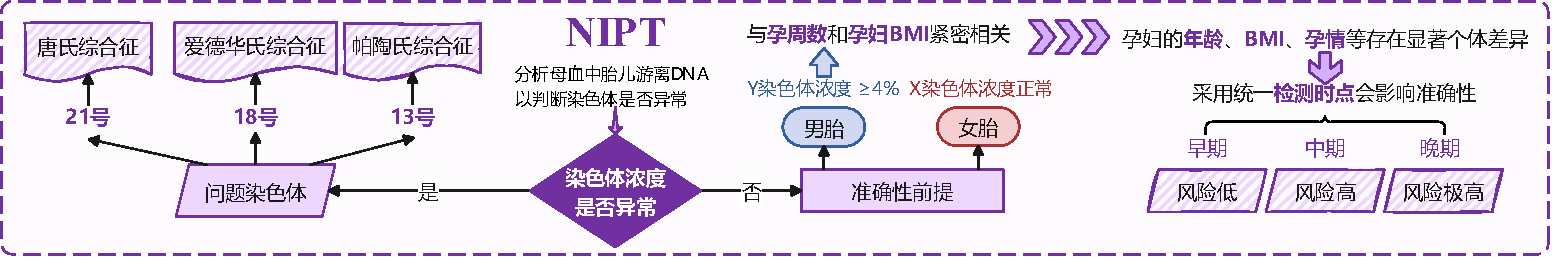
\includegraphics[width=\textwidth]{figs/1前置/问题背景.pdf}
	\caption{问题背景示意图}
\end{figure}

\section{问题重述}

\textbf{问题一:}分析胎儿染色体浓度与孕妇孕周数和身体质量指数等指标的相互关系,并建立相应的关系模型。

\textbf{问题二:}针对男胎孕妇,依据其身体质量指数进行分组,确定各组的最佳无创产前检测时点以使潜在风险最小,并分析检测误差造成的影响。

\textbf{问题三:}考虑身高,体重,年龄等多重因素与检测误差,根据男胎孕妇的身体质量指数进行分组,并给出每组的最佳无创产前检测时点,以最小化孕妇潜在风险并顾及Y染色体浓度达标比例。

\textbf{问题四:}建立女胎染色体异常的判定方法,运用Z值,GC含量,读段数及身体质量指数等多种因素,以识别21号,18号和13号染色体的非整倍体异常。


\section{问题分析(需修改)}

针对问题一,该问题涉及两个层面,其一是定性关系的判断,其二是定量规律的分析与预测。表面风化与玻璃类型、纹饰、颜色均为分类变量,它们之间的关联性分析适合采用非参数的卡方检验。风化对化学成分含量的影响则需要分组进行统计比较,通过观察含量分布的变化来识别规律。由于缺乏同一文物风化前后的成对数据,直接建立回归预测模型存在困难,因此分析的重点在于依据风化机理,构建一个基于平均变化率的风化系数模型,用以反推风化前的化学成分。

针对问题二,该问题需要从监督学习与无监督学习两个角度展开。高钾与铅钡玻璃的分类规律研究是一个典型的二分类问题,可以基于探索性数据分析发现的关键化学成分,构建支持向量机等分类模型,并对模型进行解释。

针对问题三,该问题是分类模型的实际应用与可靠性验证。分析的核心在于构建一个泛化能力强且稳健的分类器。这需要比较多种模型架构,并论证选择支持向量机的合理性。为使模型性能最优化,需要采用改进遗传算法等智能优化算法进行超参数寻优。最终的鉴别结果需要通过数据扰动和模型参数敏感性分析的双重检验,以证明其结论并非偶然,而是具有高度的可靠性。

针对问题四,该问题要求探寻不同类别玻璃内部化学成分的关联结构。由于玻璃成分数据具有总和恒定的特性,直接计算相关系数会产生误导,因此必须首先采用中心化对数比变换来消除此统计约束。直接计算相关系数会产生误导,因此必须首先采用中心化对数比变换来消除此统计约束。

全文框架如\cref{fig:全文框架}所示:

\begin{figure}[H]
	\centering
	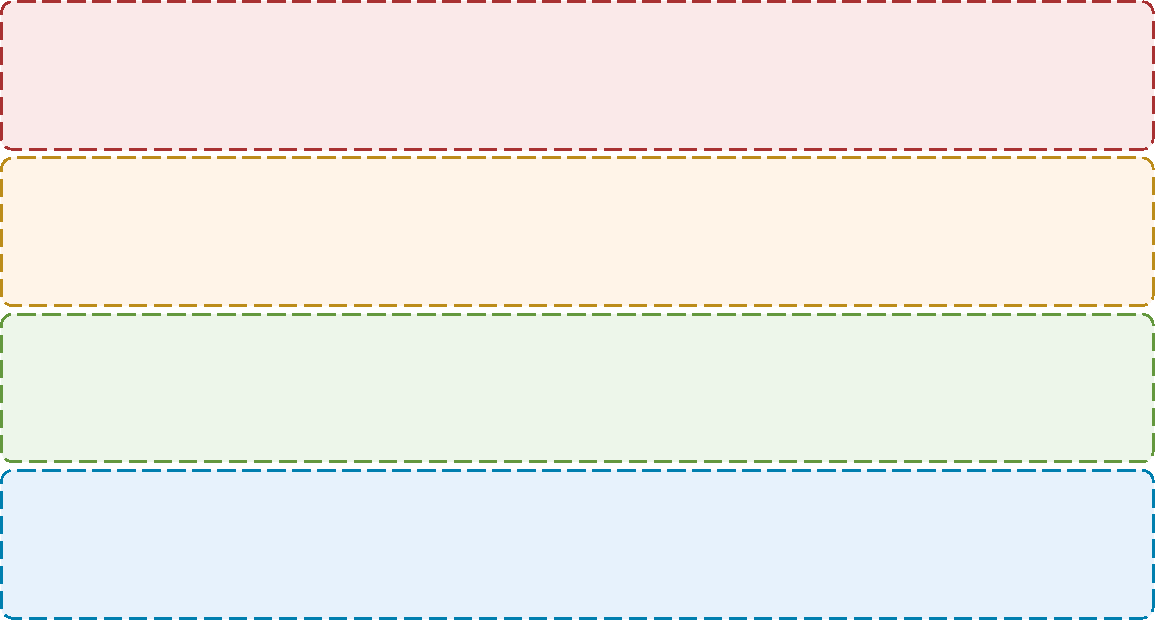
\includegraphics[width=\textwidth]{figs/1前置/全文框架.pdf}
	\caption{全文框架示意图}
	\label{fig:全文框架}
\end{figure}


\section{模型假设(需修改)}
为保证模型构建的合理性与分析过程的严谨性,我们提出以下基本假设。
\begin{enumerate}
	\item 所有用于分析的数据均为成分总和在百分之八十五至一百零五区间的有效数据。
	\item 数据中的空白项表示该化学成分未被检测到其含量可视为零。
	\item 同一类型玻璃的风化过程与化学成分变化规律具有统计上的一致性。
	\item 文物的化学成分组合能够有效地区分高钾玻璃与铅钡玻璃两大类别。
	\item 同一文物多个采样点的平均化学成分可以代表该文物的整体特征用于亚类划分。
	\item 化学成分间的偏相关关系能够反映其在玻璃配方或制作工艺中的直接关联。
	\item 化学成分间的偏相关关系能够反映其在玻璃配方或制作工艺中的直接关联。
\end{enumerate}

\section{符号说明(需修改)}
本文后续章节中所使用的主要数学符号及其说明如表所示。

\begin{table}[H]
	\centering
	\caption{符号说明表}
	\begin{tabular}{ll}
		\toprule
		\textbf{符号}                        & \textbf{说明}                     \\
		\midrule
		$k_{t,j}$                          & $t$类玻璃中$j$成分的风化系数               \\
		$\bar{C}_{t,j,\text{weathered}}$   & $t$类玻璃风化样本中$j$成分的平均含量           \\
		$\bar{C}_{t,j,\text{unweathered}}$ & $t$类玻璃未风化样本中$j$成分的平均含量          \\
		$C'_{\text{unweathered}, j}$       & 某一样本风化前$j$成分的预测含量               \\
		$\boldsymbol{w}, b$                & 支持向量机分类超平面的法向量与位移项              \\
		$C$                                & 支持向量机的正则化系数                     \\
		$\gamma$                           & 径向基核函数的参数                       \\
		$\xi_i$                            & 支持向量机的松弛变量                      \\
		$CV$                               & 变异系数,用于衡量数据的相对离散程度              \\
		$\text{clr}(\boldsymbol{x})$       & 对样本向量$\boldsymbol{x}$进行中心化对数比变换 \\
		$S$                                & 样本协方差矩阵                         \\
		$\Theta$                           & 精度矩阵,即逆协方差矩阵                    \\
		$\lambda$                          & 图套索算法的正则化参数                     \\
		$\rho_{ij \cdot \text{rest}}$      & 变量$i$和$j$之间的偏相关系数               \\
		$S$                                & 样本协方差矩阵                         \\
		$\Theta$                           & 精度矩阵,即逆协方差矩阵                    \\
		$\lambda$                          & 图套索算法的正则化参数                     \\
		$\rho_{ij \cdot \text{rest}}$      & 变量$i$和$j$之间的偏相关系数               \\
		\bottomrule
	\end{tabular}
\end{table}
\section{模型准备}

为了后续模型的建立与求解,本文进行如下模型准备,即数据清洗、数据量化等。具体机制如\cref{fig:模型准备机制}所示。

\begin{figure}[h!]
\centering
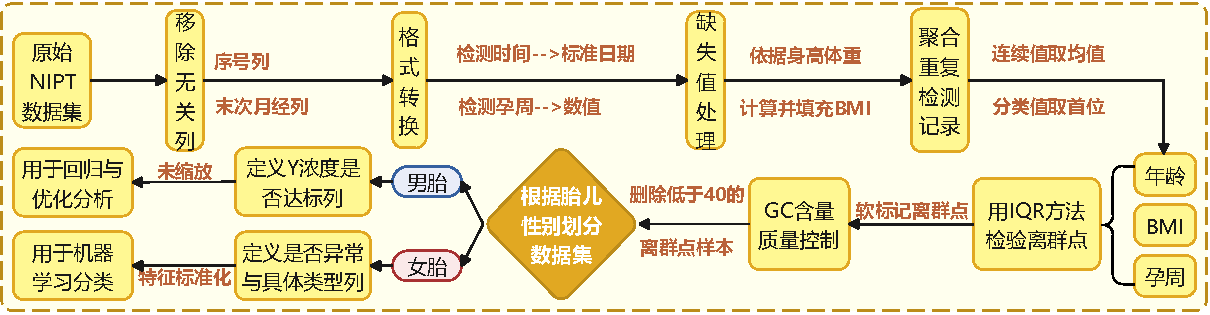
\includegraphics[width=1\textwidth]{figs/2模型准备/模型准备.pdf}
\caption{模型准备机制}
\label{fig:模型准备机制}
\end{figure}

\subsection{数据清洗}

\subsubsection{缺失值处理与数据整合}
为简化数据集,我们移除了与建模任务无直接关联的序号列。随后,我们对数据集中各变量进行缺失值统计,发现末次月经时间列存在部分数据缺失。末次月经时间的主要功能为推算孕周,而数据集中已包含更为直接的检测孕周列,故将其移除。

为使原始特征能够用于定量分析,我们需要将其转化为标准的数值格式。对于纯数字格式的检测时间列,我们将其转换为标准的日期时间格式;对于文本格式的检测孕周列,我们转换为可计算的浮点数值,例如十二周加三天转化为12.43周。对于孕妇BMI指标列中的缺失值,我们利用同一条记录的身高与体重数据,依据身体质量指数的官方计算公式进行填充,该公式如下所示
\begin{equation}
BMI = \frac{Weight(kg)}{Height(m)^2}
\label{eq:bmi}
\end{equation}
与使用均值或中位数等统计量填充相比,利用已有数据进行计算能最大限度地保持数据的真实性。



完成基础清洗与计算后,数据集内核心特征的整体分布如\cref{fig:核心特征分布}所示。该图展示了孕妇年龄,孕妇BMI与检测孕周三个变量的分布状况。从图中可以看出样本的年龄主要集中在25至35岁之间,孕妇BMI分布的峰值位于30附近,证实了样本多为高BMI的地区特征。检测孕周则在12至25周之间呈现多个峰值,表明了检测时间点的集中性。

\begin{figure}[h!]
\centering
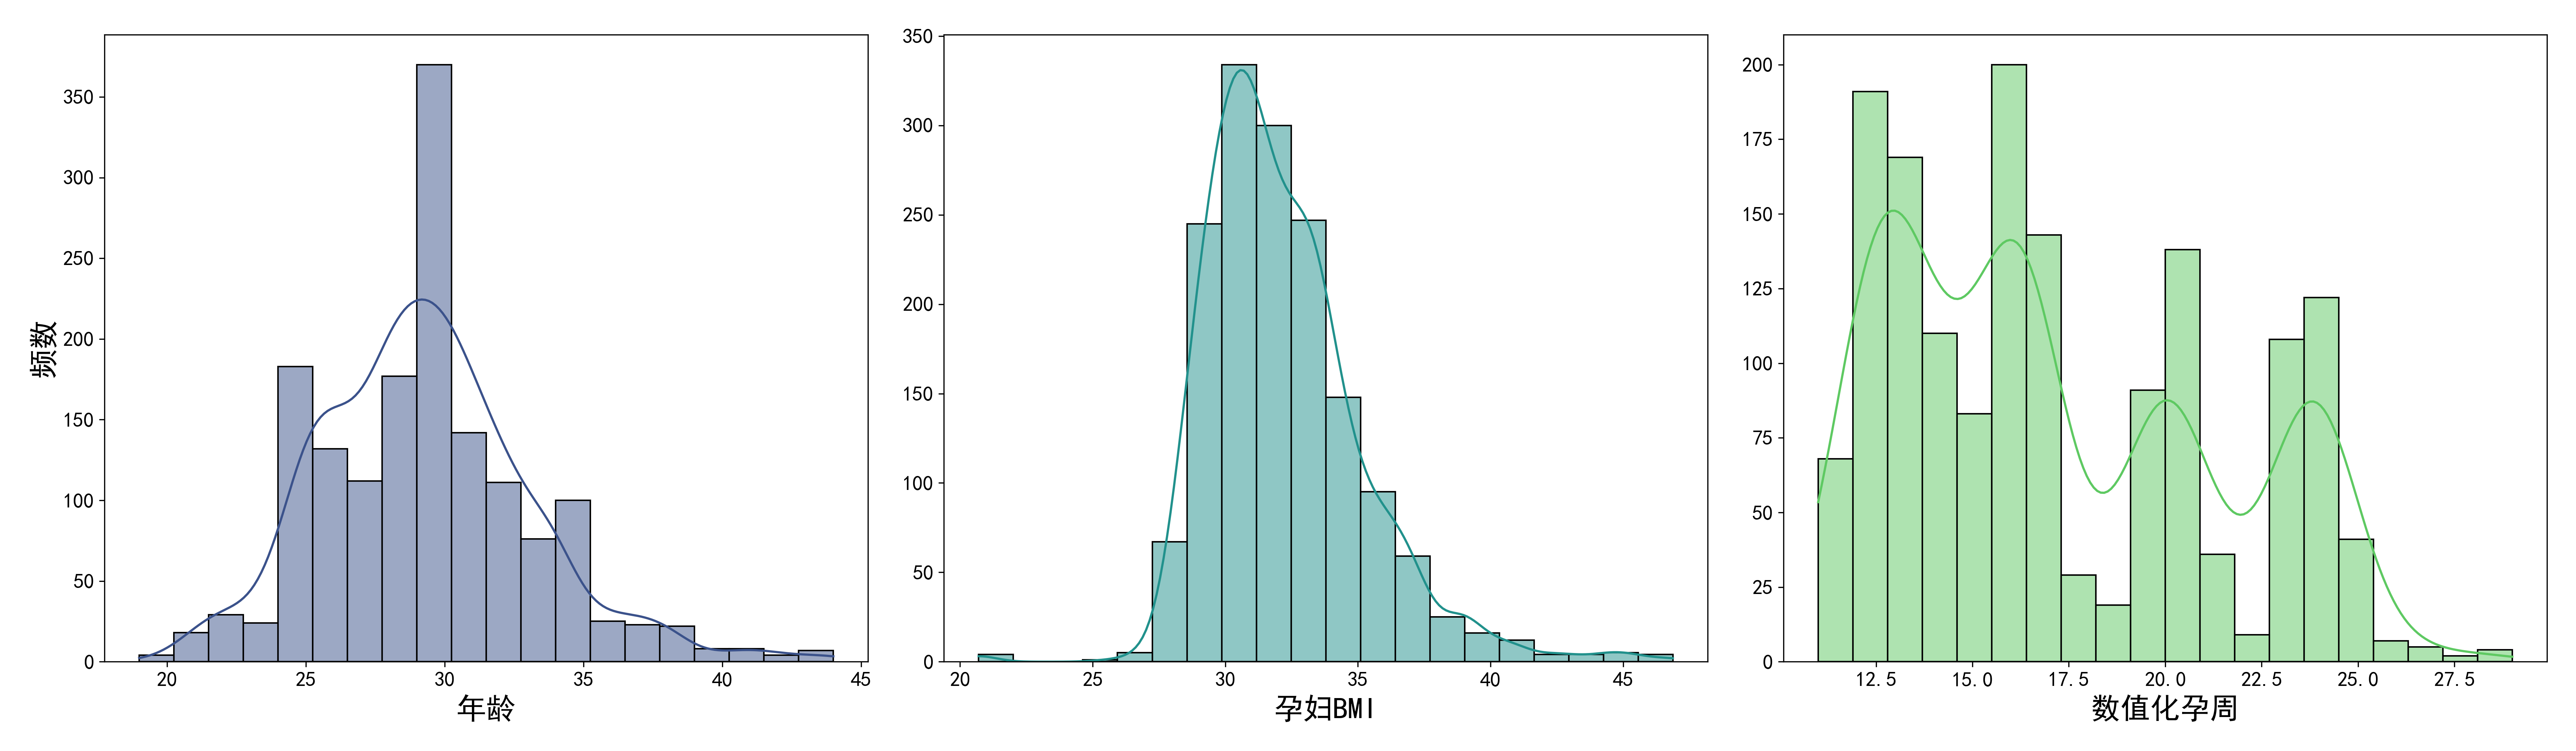
\includegraphics[width=1\textwidth]{figs/2模型准备/图1_核心特征分布.png}
\caption{核心特征分布}
\label{fig:核心特征分布}
\end{figure}

题目中提到存在对同一孕妇进行重复检测的情况,这导致了数据冗余。为消除此冗余,我们以孕妇代码与检测抽血次数为唯一标识,对同一抽血样本的多次检测记录进行数据整合。整合时,对于连续性测量指标,取其算术平均值以减小单次测量的随机误差影响;对于分类性状态指标,则保留其首次出现的值。

\cref{fig:整合效果对比}展示了数据整合前后的样本数量变化。如左图所示,处理前单个孕妇的样本记录数最高可达9条,多数孕妇具有1至6条记录。经过整合处理后,转变为每次抽血对应唯一记录的形式。如右图所示,单个孕妇的有效检测次数减少至1至5次,大部分孕妇只有4次有效检测,从而消除了冗余信息。

根据题目说明,原始数据中存在同一孕妇多次采血多次检测或一次采血多次检测的情况,这种情况造成了数据冗余。为消除此冗余并为每个样本建立唯一的检测记录,本文以孕妇代码与检测抽血次数的组合为标识,对重复的检测条目进行聚合处理。在聚合过程中,对于连续型测量指标,采用算术平均值以平滑单次测量的随机波动。对于分类性质的状态指标,则保留其初次记录的值。

该聚合过程的效果通过\cref{fig:整合效果对比}中的前后对比得以展示。左图显示在处理前,单个孕妇对应的所有样本的所有检测记录数从1条至9条不等,其中多数孕妇具有3至6条记录。经过聚合处理后,如右图所示,每位孕妇的有效检测次数范围缩小至1至5次,其中具有4次有效检测的孕妇数量最多。


\begin{figure}[h!]
    \centering
    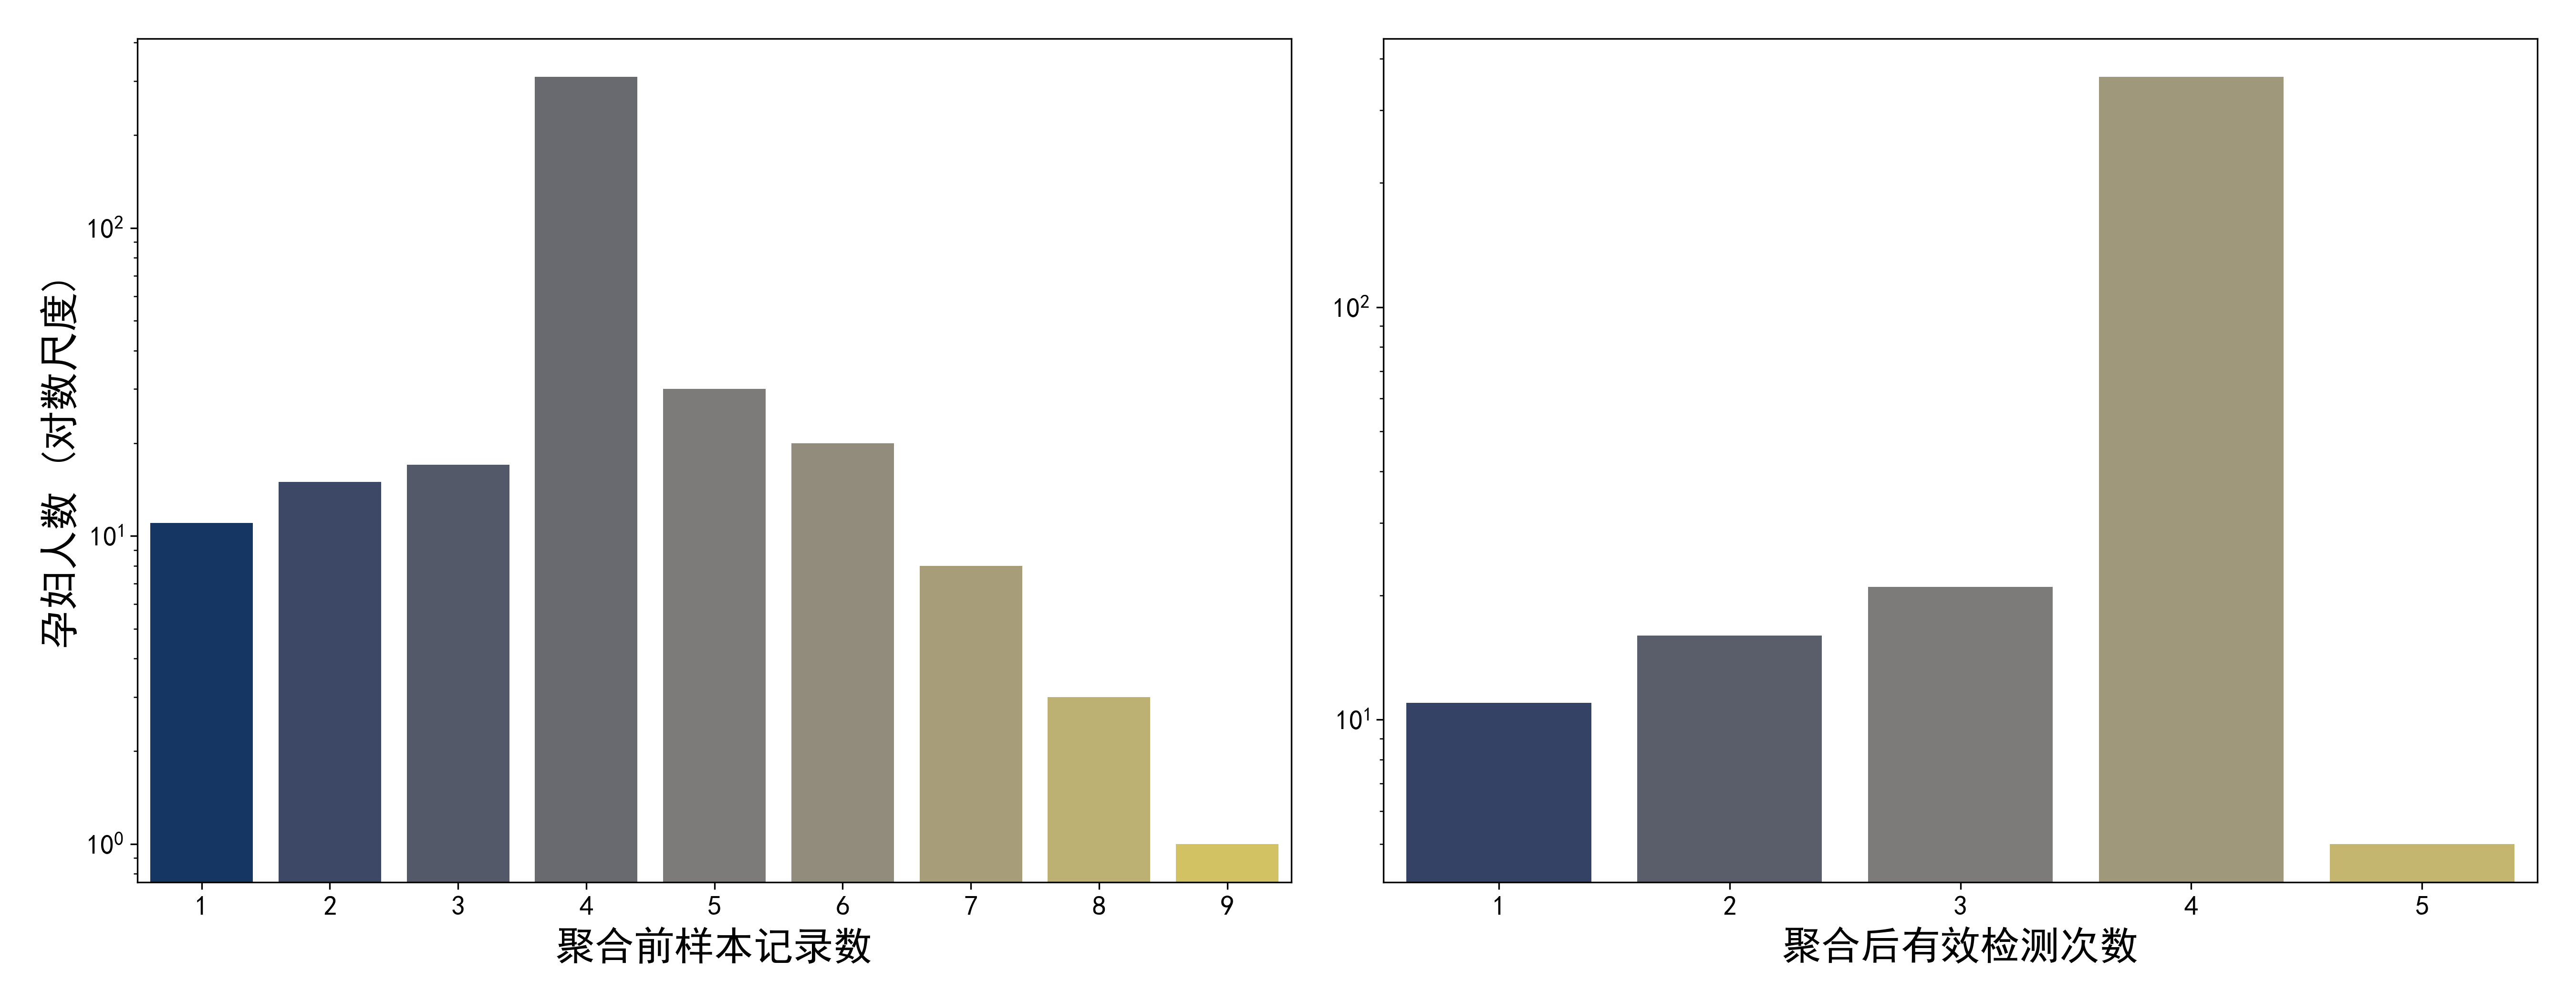
\includegraphics[width=1\textwidth]{figs/2模型准备/图2_聚合效果对比.png}
    \caption{数据整合效果对比}
    \label{fig:整合效果对比}
\end{figure}

\subsubsection{异常值处理}

我们首先针对年龄,孕妇BMI与孕周这三个核心特征执行四分位距法检验。对于识别出的离群点,本文采用软标记方法,即在数据集中新增一列用以标记样本是否为离群点,而不直接删除样本记录。离群点可能代表了真实存在的极端生理状况或数据录入错误,采用软标记策略为后续建模提供了灵活性。\cref{fig:IQR离群点分析}展示了离群点分析的过程,图中每个子图的小提琴形状表示了数据的分布,红色的圆点则标记出被标准四分位距准则判定为离群点的样本。图中可见,年龄的离群点主要分布在40岁以上的高龄区间,孕妇BMI的离群点则同时出现在低于20的低值区域与高于40的高值区域,而孕周的离群点相对较少。

\begin{figure}[h!]
\centering
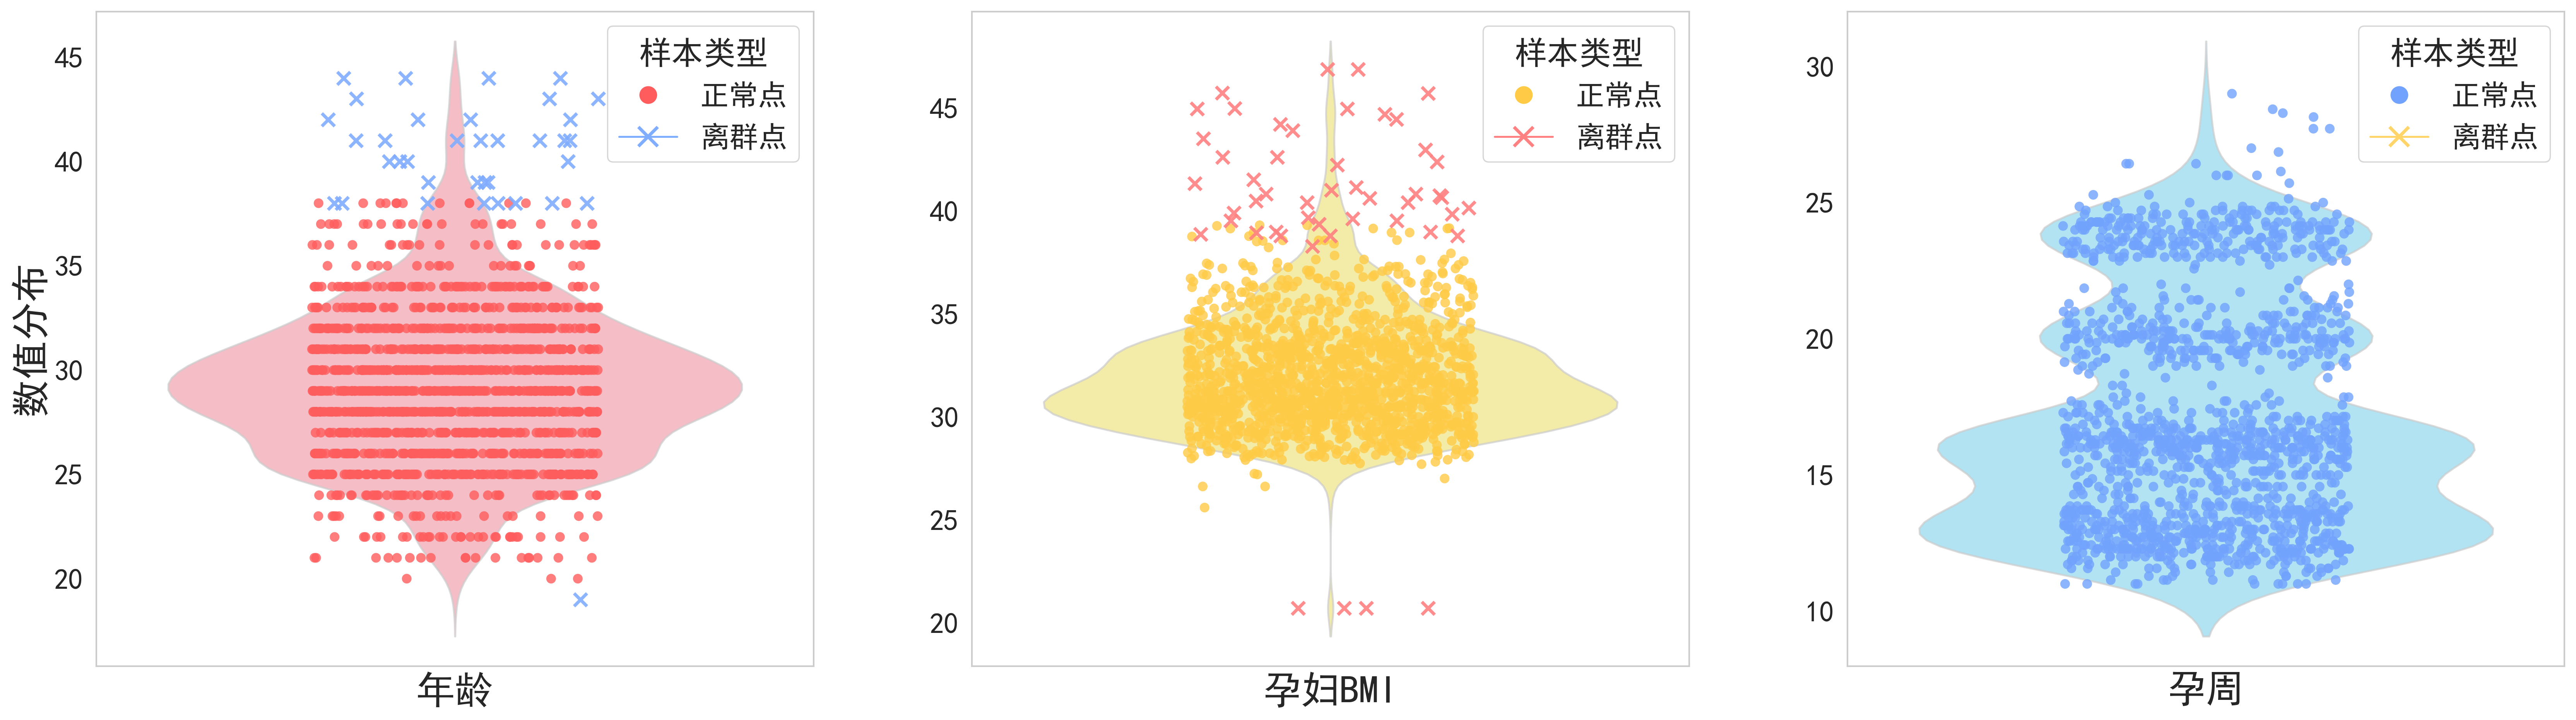
\includegraphics[width=1\textwidth]{figs/2模型准备/图3_IQR离群点分析.png}
\caption{IQR离群点分析}
\label{fig:IQR离群点分析}
\end{figure}

其次我们对GC含量进行质量控制。GC含量是衡量测序质量的重要指标。处理过程结合了统计学检验与业务规则,先对GC含量列执行标准的1.5倍四分位距检验以识别出所有统计学上的离群点。然后,仅将这些离群点中数值低于40\%的样本从数据集中直接删除。此方法能够剔除那些不仅在统计上异常,且低于业务经验常规下限的低质量测序样本。\cref{fig:GC含量离群点分析}展示了处理后的数据,其中直方图展示了GC含量的整体分布形态近似正态分布,频数在0.400处达到峰值,绝大多数样本的GC含量分布在0.395至0.405之间,分布集中,数据质量较高。

\begin{figure}[h!]
\centering
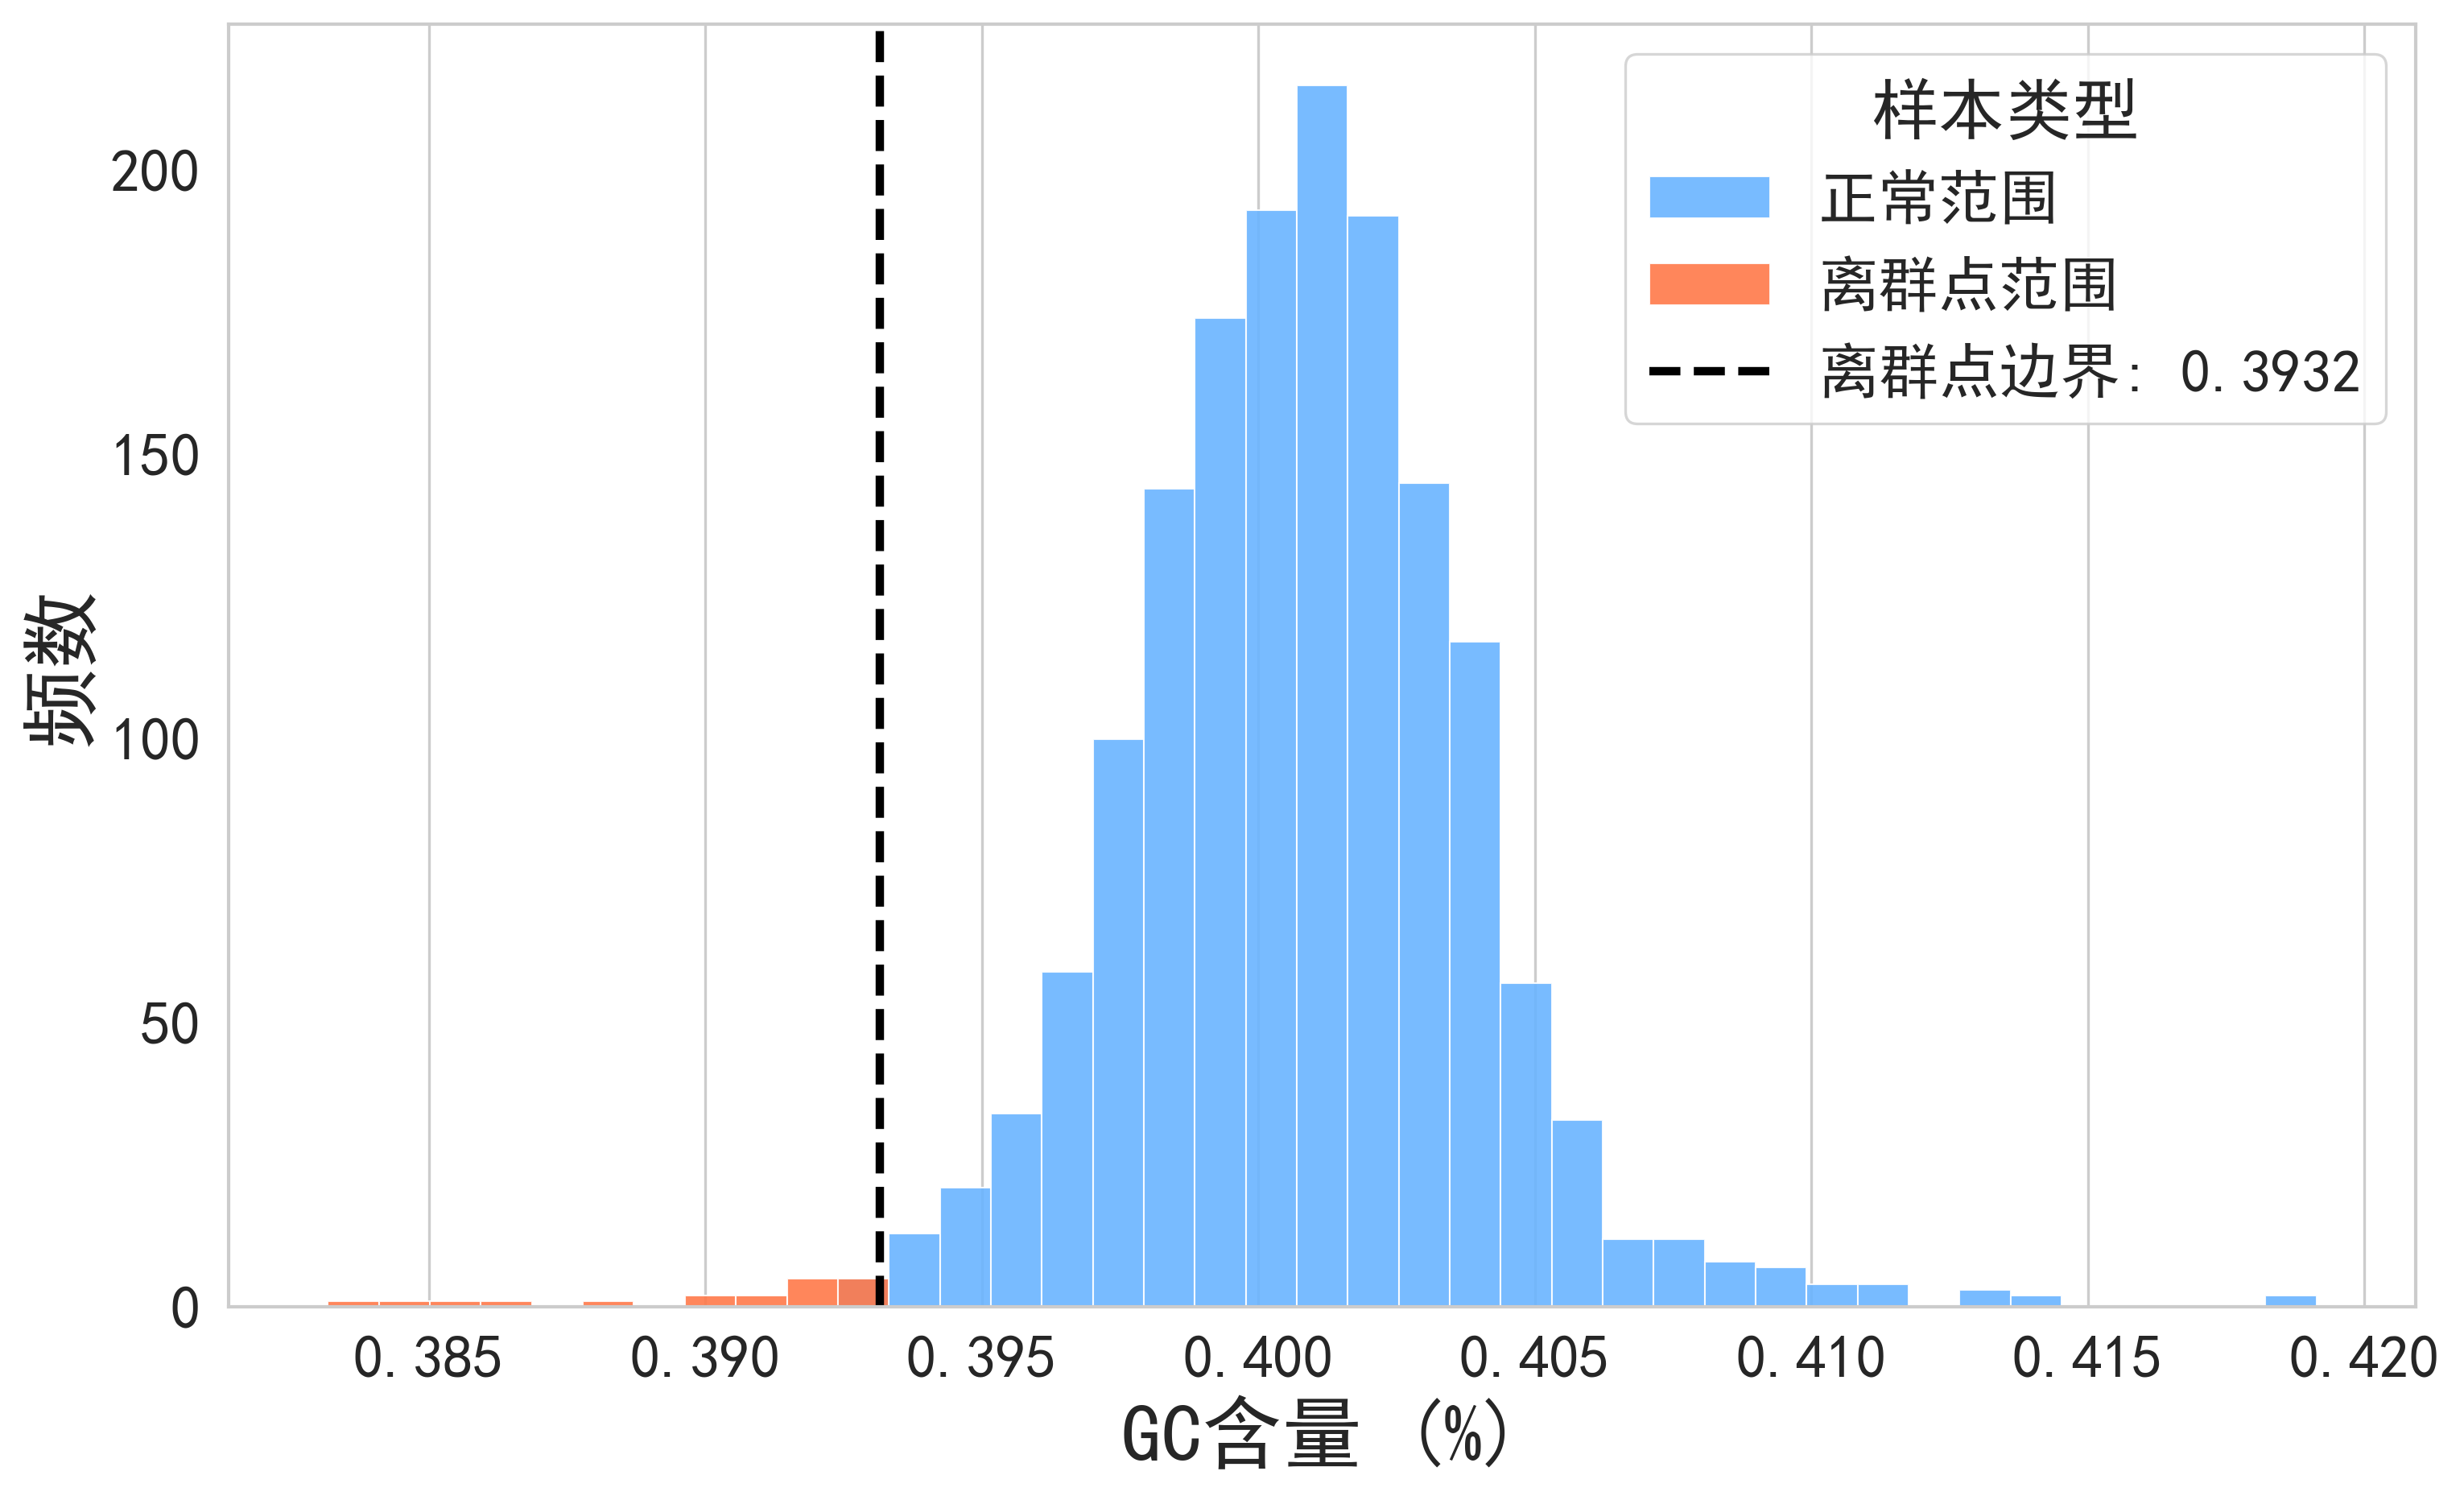
\includegraphics[width=\textwidth]{figs/2模型准备/图4_GC含量离群点分析.png}
\caption{GC含量离群点分析}
\label{fig:GC含量离群点分析}
\end{figure}

\subsection{数据量化}
为了便于后续相关数学模型的建立与求解,增强可理解性,我们进一步进行了数据量化。

针对不同问题,我们构建了相应的目标变量。对于男胎数据,依据题目定义的4\%阈值,我们创建了“Y浓度是否达标”的二元分类变量。对于女胎数据,则基于染色体的非整倍体列中空白即为无异常的定义,创建了“是否异常”以及各类异常的分类目标。\cref{fig:染色体异常类型分布}展示了女胎样本中正常与各类异常样本的数量分布。图中可见正常样本数量为488例,而18号,13号与21号染色体三体综合征的样本数量分别为45例,22例与13例。正常样本远多于异常样本,表明这是一个数据不平衡问题。

\begin{figure}[h!]
\centering
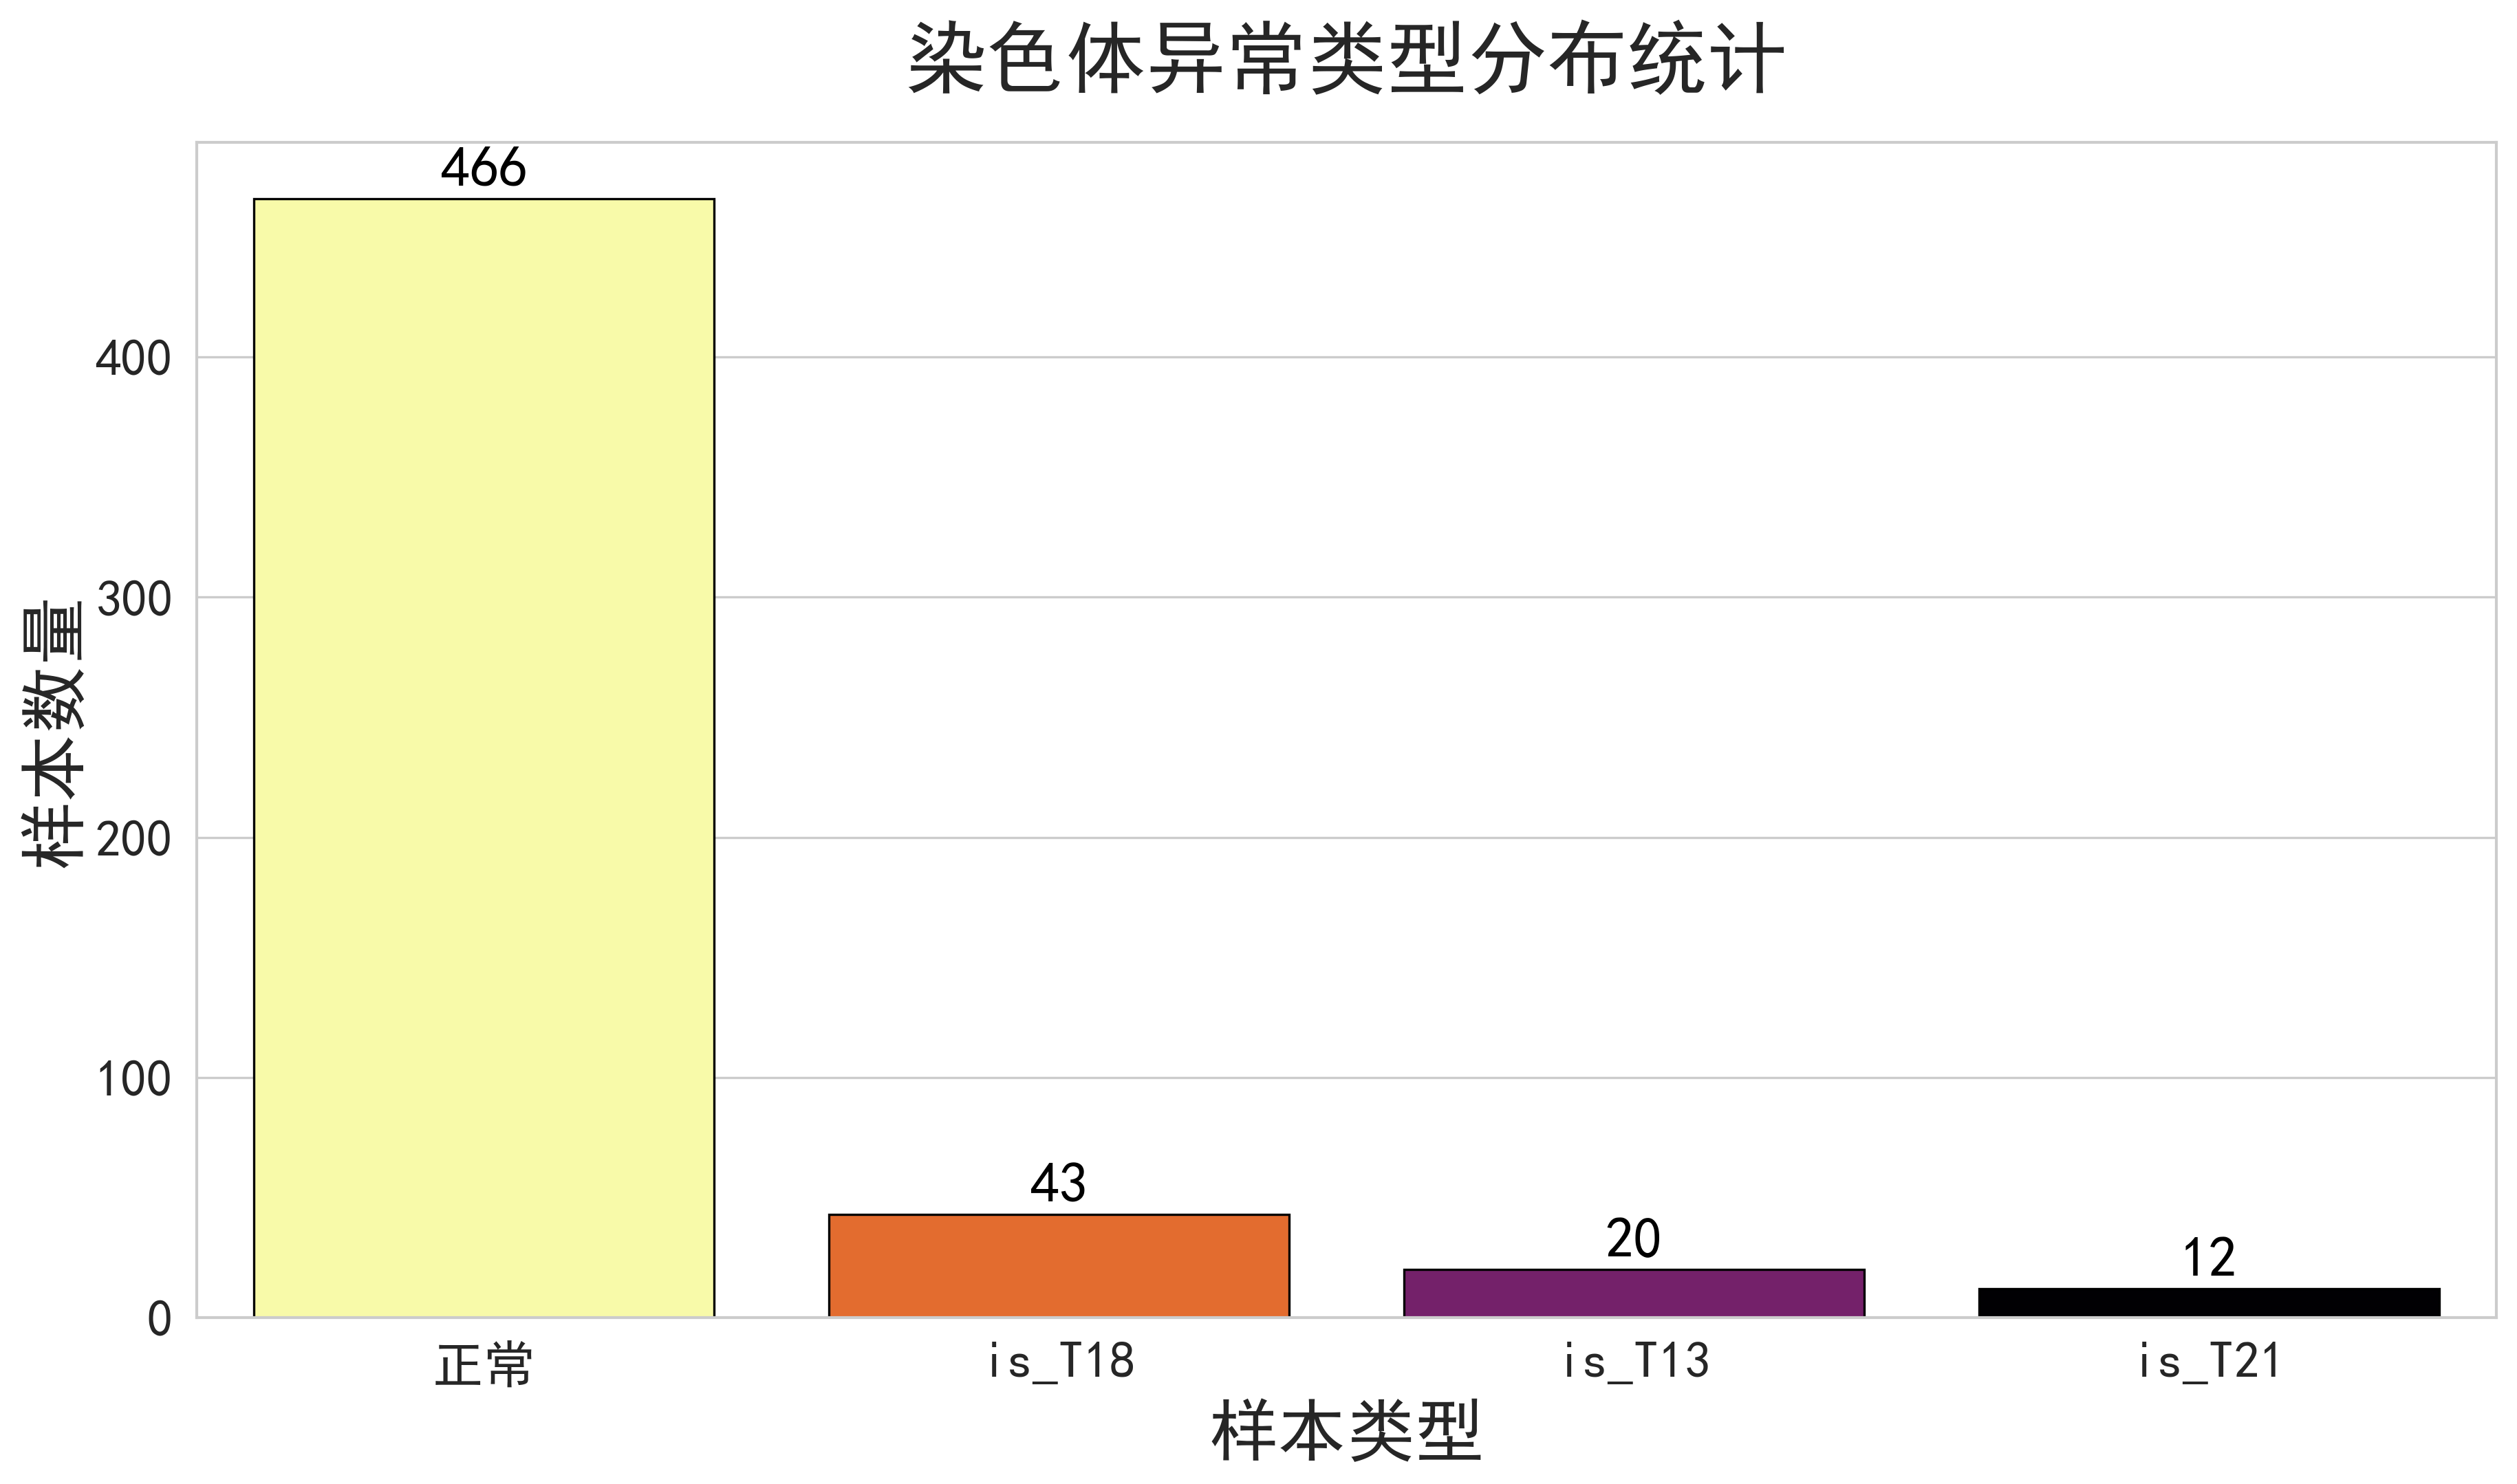
\includegraphics[width=0.8\textwidth]{figs/2模型准备/图5_染色体异常类型分布.png}
\caption{染色体异常类型分布}
\label{fig:染色体异常类型分布}
\end{figure}

考虑到问题四需要使用机器学习分类模型,我们仅针对女胎数据的所有数值型预测特征应用了标准化处理。标准化将所有特征转换到同一尺度,其计算方法如下
\begin{equation}
z = \frac{x - \mu}{\sigma}
\label{eq:standardization}
\end{equation}
其中 $x$ 为原始值,$\mu$ 为特征均值,$\sigma$ 为特征标准差。此操作避免了模型的训练过程被原始读段数等具有极大数值范围的特征所主导,使模型能够更稳定地学习所有特征的贡献。男胎数据因主要用于回归和优化分析,保留其原始数值的物理意义更为重要,故不进行缩放。\cref{fig:所有数值特征缩放效果对比}展示了女胎数据中所有数值型预测变量在缩放前后的分布对比。每个子图呈现了同一特征在处理前后的分布形态,处理前各变量的分布中心与尺度范围各不相同,而经过标准化处理后,所有变量的分布均被调整至以0为中心,具有相似的尺度,这为后续机器学习模型的训练提供了同质化的输入。

\begin{figure}[h!]
\centering
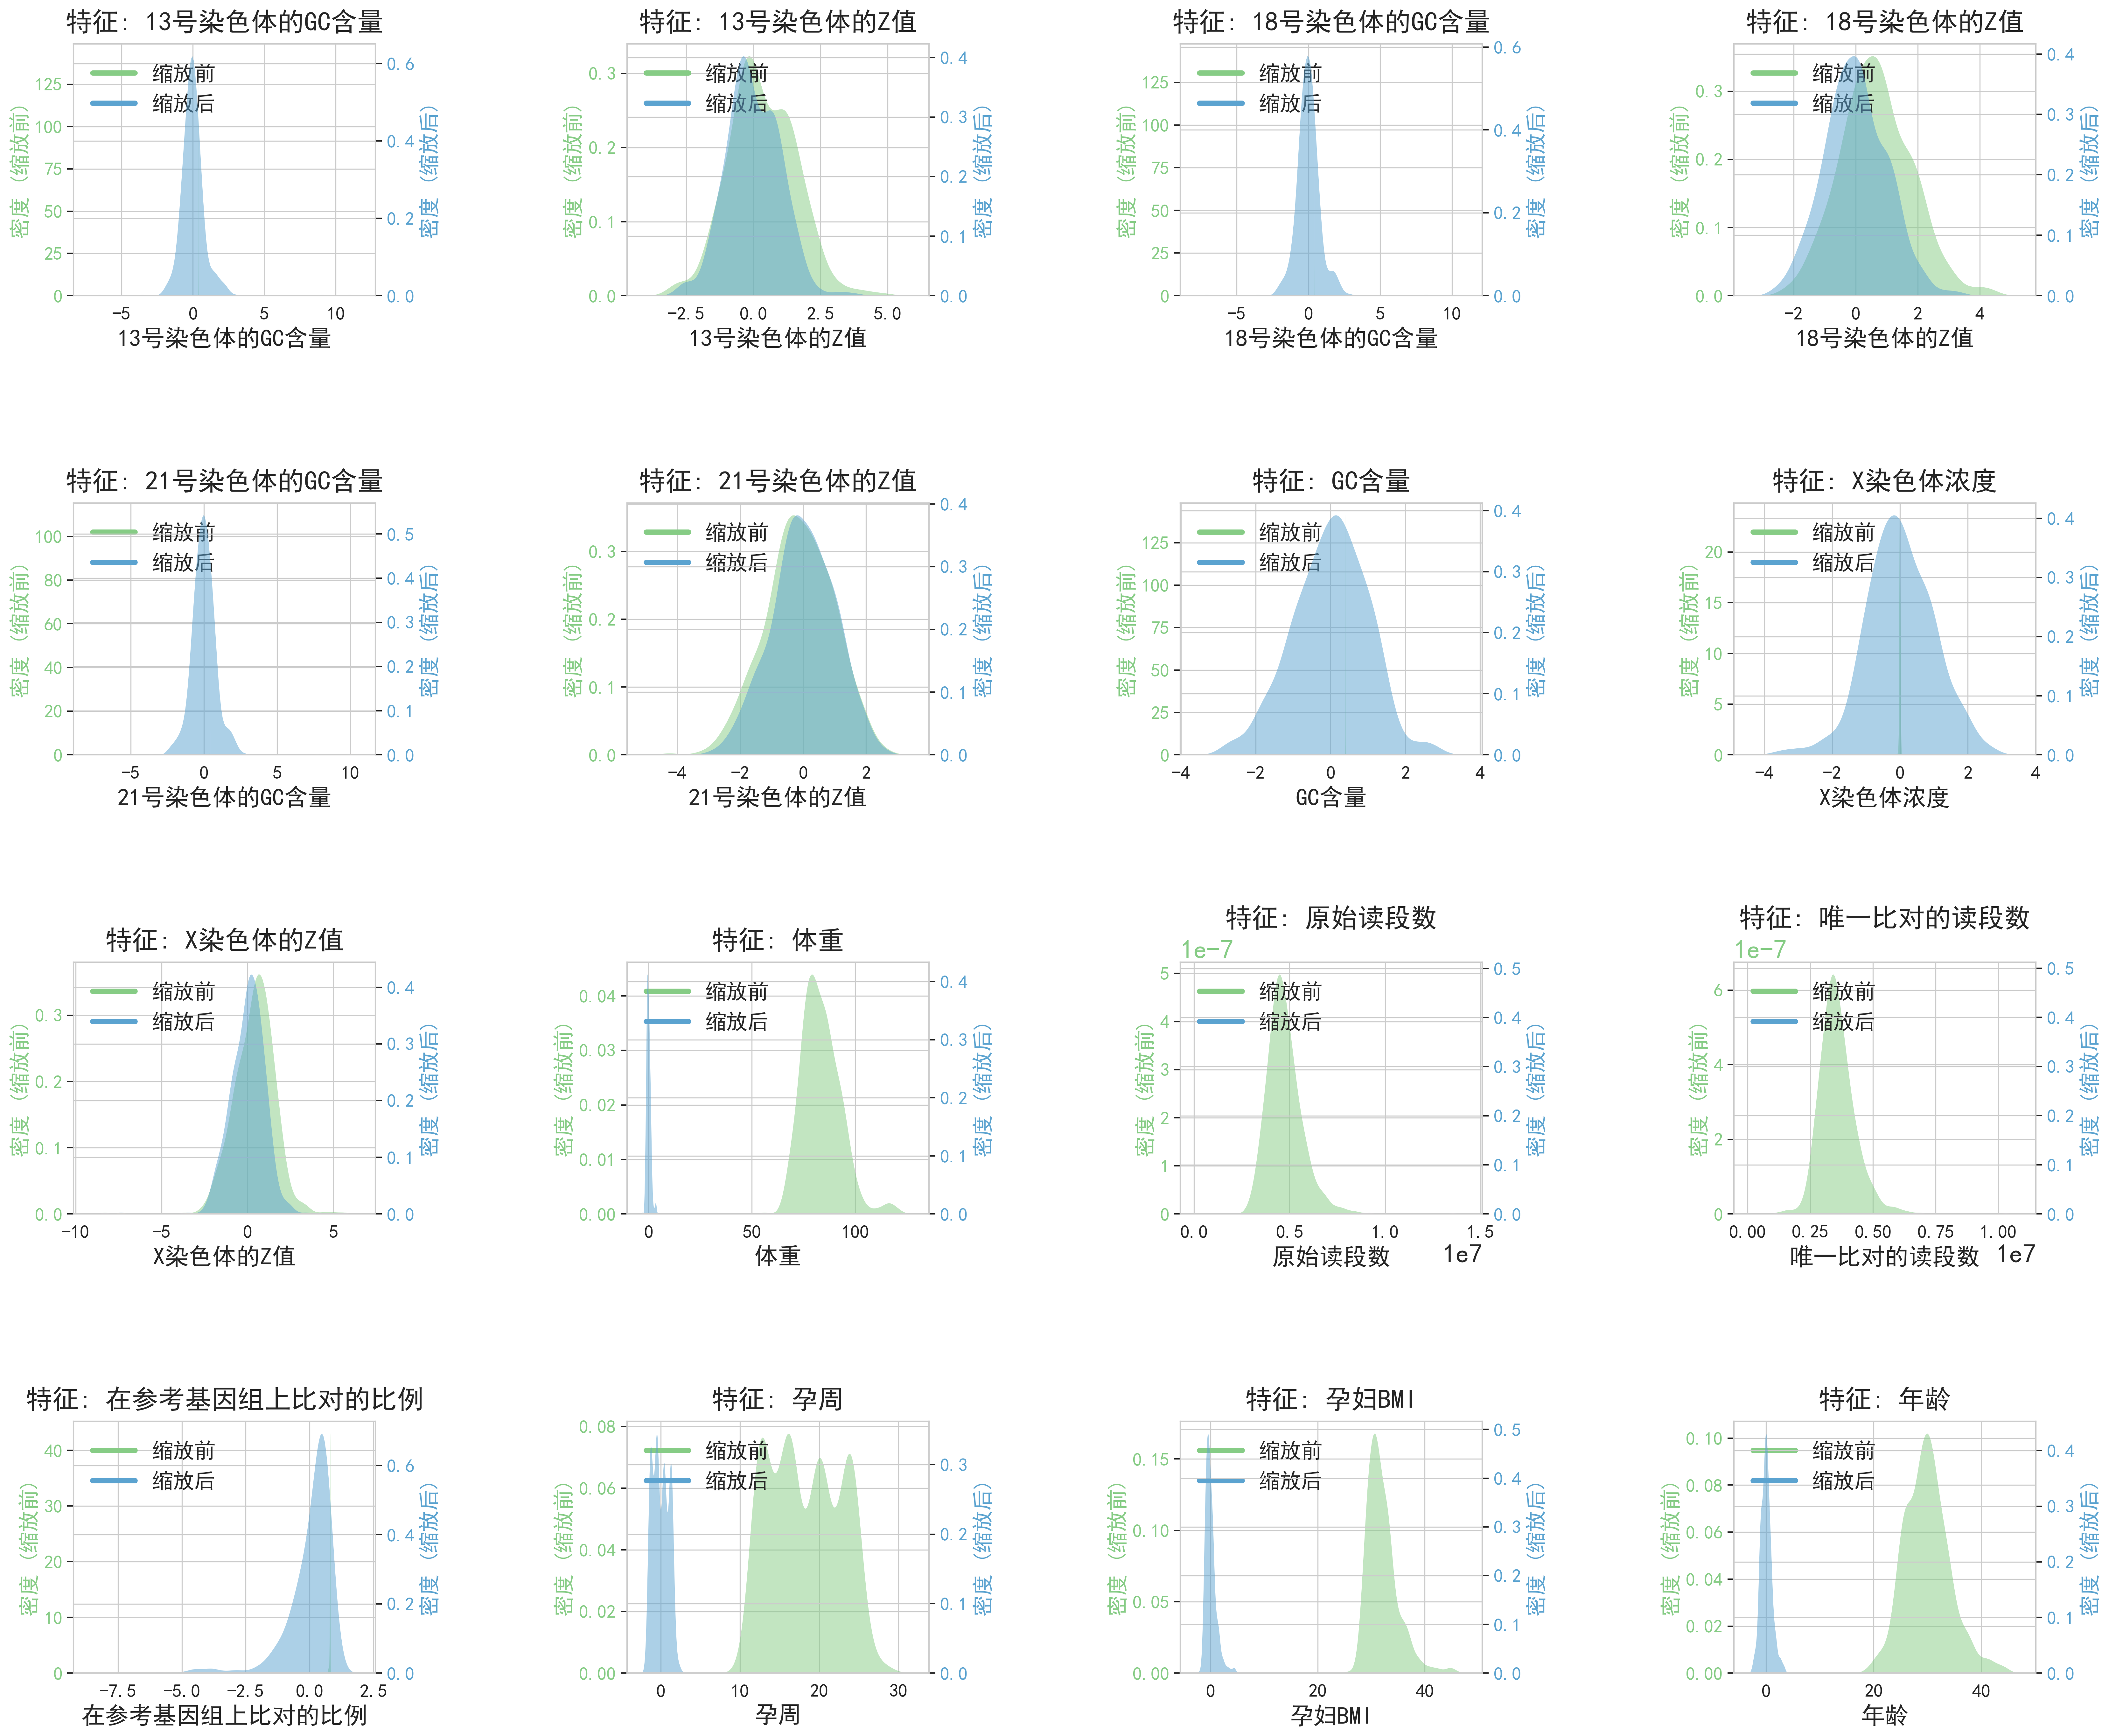
\includegraphics[width=1\textwidth]{figs/2模型准备/图6_特征缩放效果对比.png}
\caption{所有数值特征缩放效果对比}
\label{fig:数值特征缩放效果对比}
\end{figure}


此外,我们还构建了部分衍生特征。我们依据题目对风险的定义,创建了与孕周对应的风险等级特征。同时,为进行时序分析,还计算了每次检测距首次检测的天数。
\section{问题一:关系模型的建立与求解}
为识别影响男胎 Y 染色体浓度的主要因素并量化其作用,我们先构建最终数据集,再通过探索性分析与迭代建模建立能反映数据规律的关系模型。具体流程见 \cref{fig:关系模型的建立与求解流程}。

\begin{figure}[h!]
    \centering
    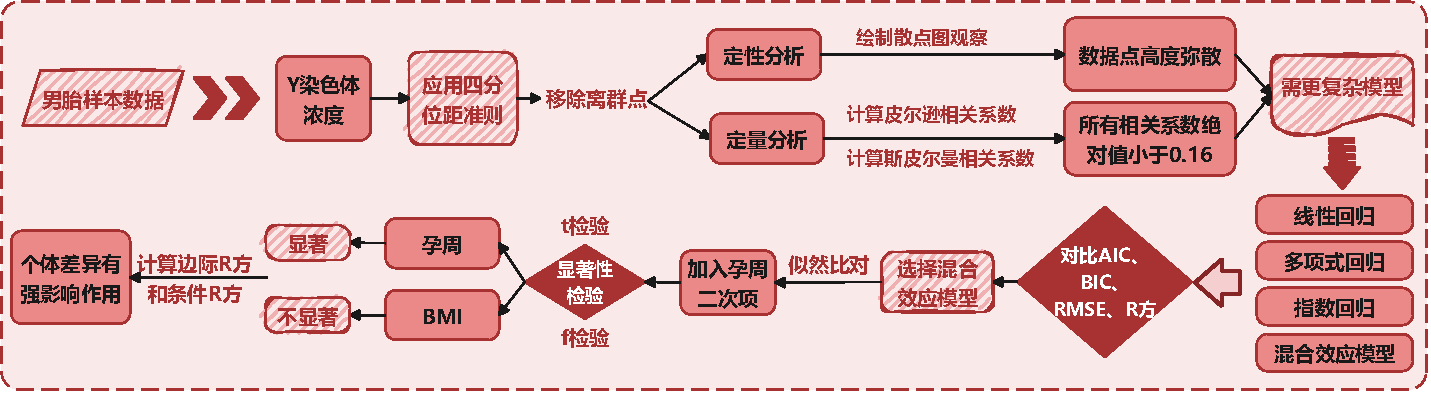
\includegraphics[width=\textwidth]{figs/3问题一/问题一.pdf}
    \caption{关系模型的建立与求解流程}
    \label{fig:关系模型的建立与求解流程}
\end{figure}

\subsection{数据准备与探索性分析}
分析始于一份经过初步处理的男胎样本数据。为保证后续建模的稳定,我们对Y染色体浓度这个核心变量应用了四分位距法进行离群点检测。在联合筛选标准下,部分包含极端值的样本记录被移除,最终形成了一个用于建模的分析数据集。

\begin{figure}[h!]
\centering
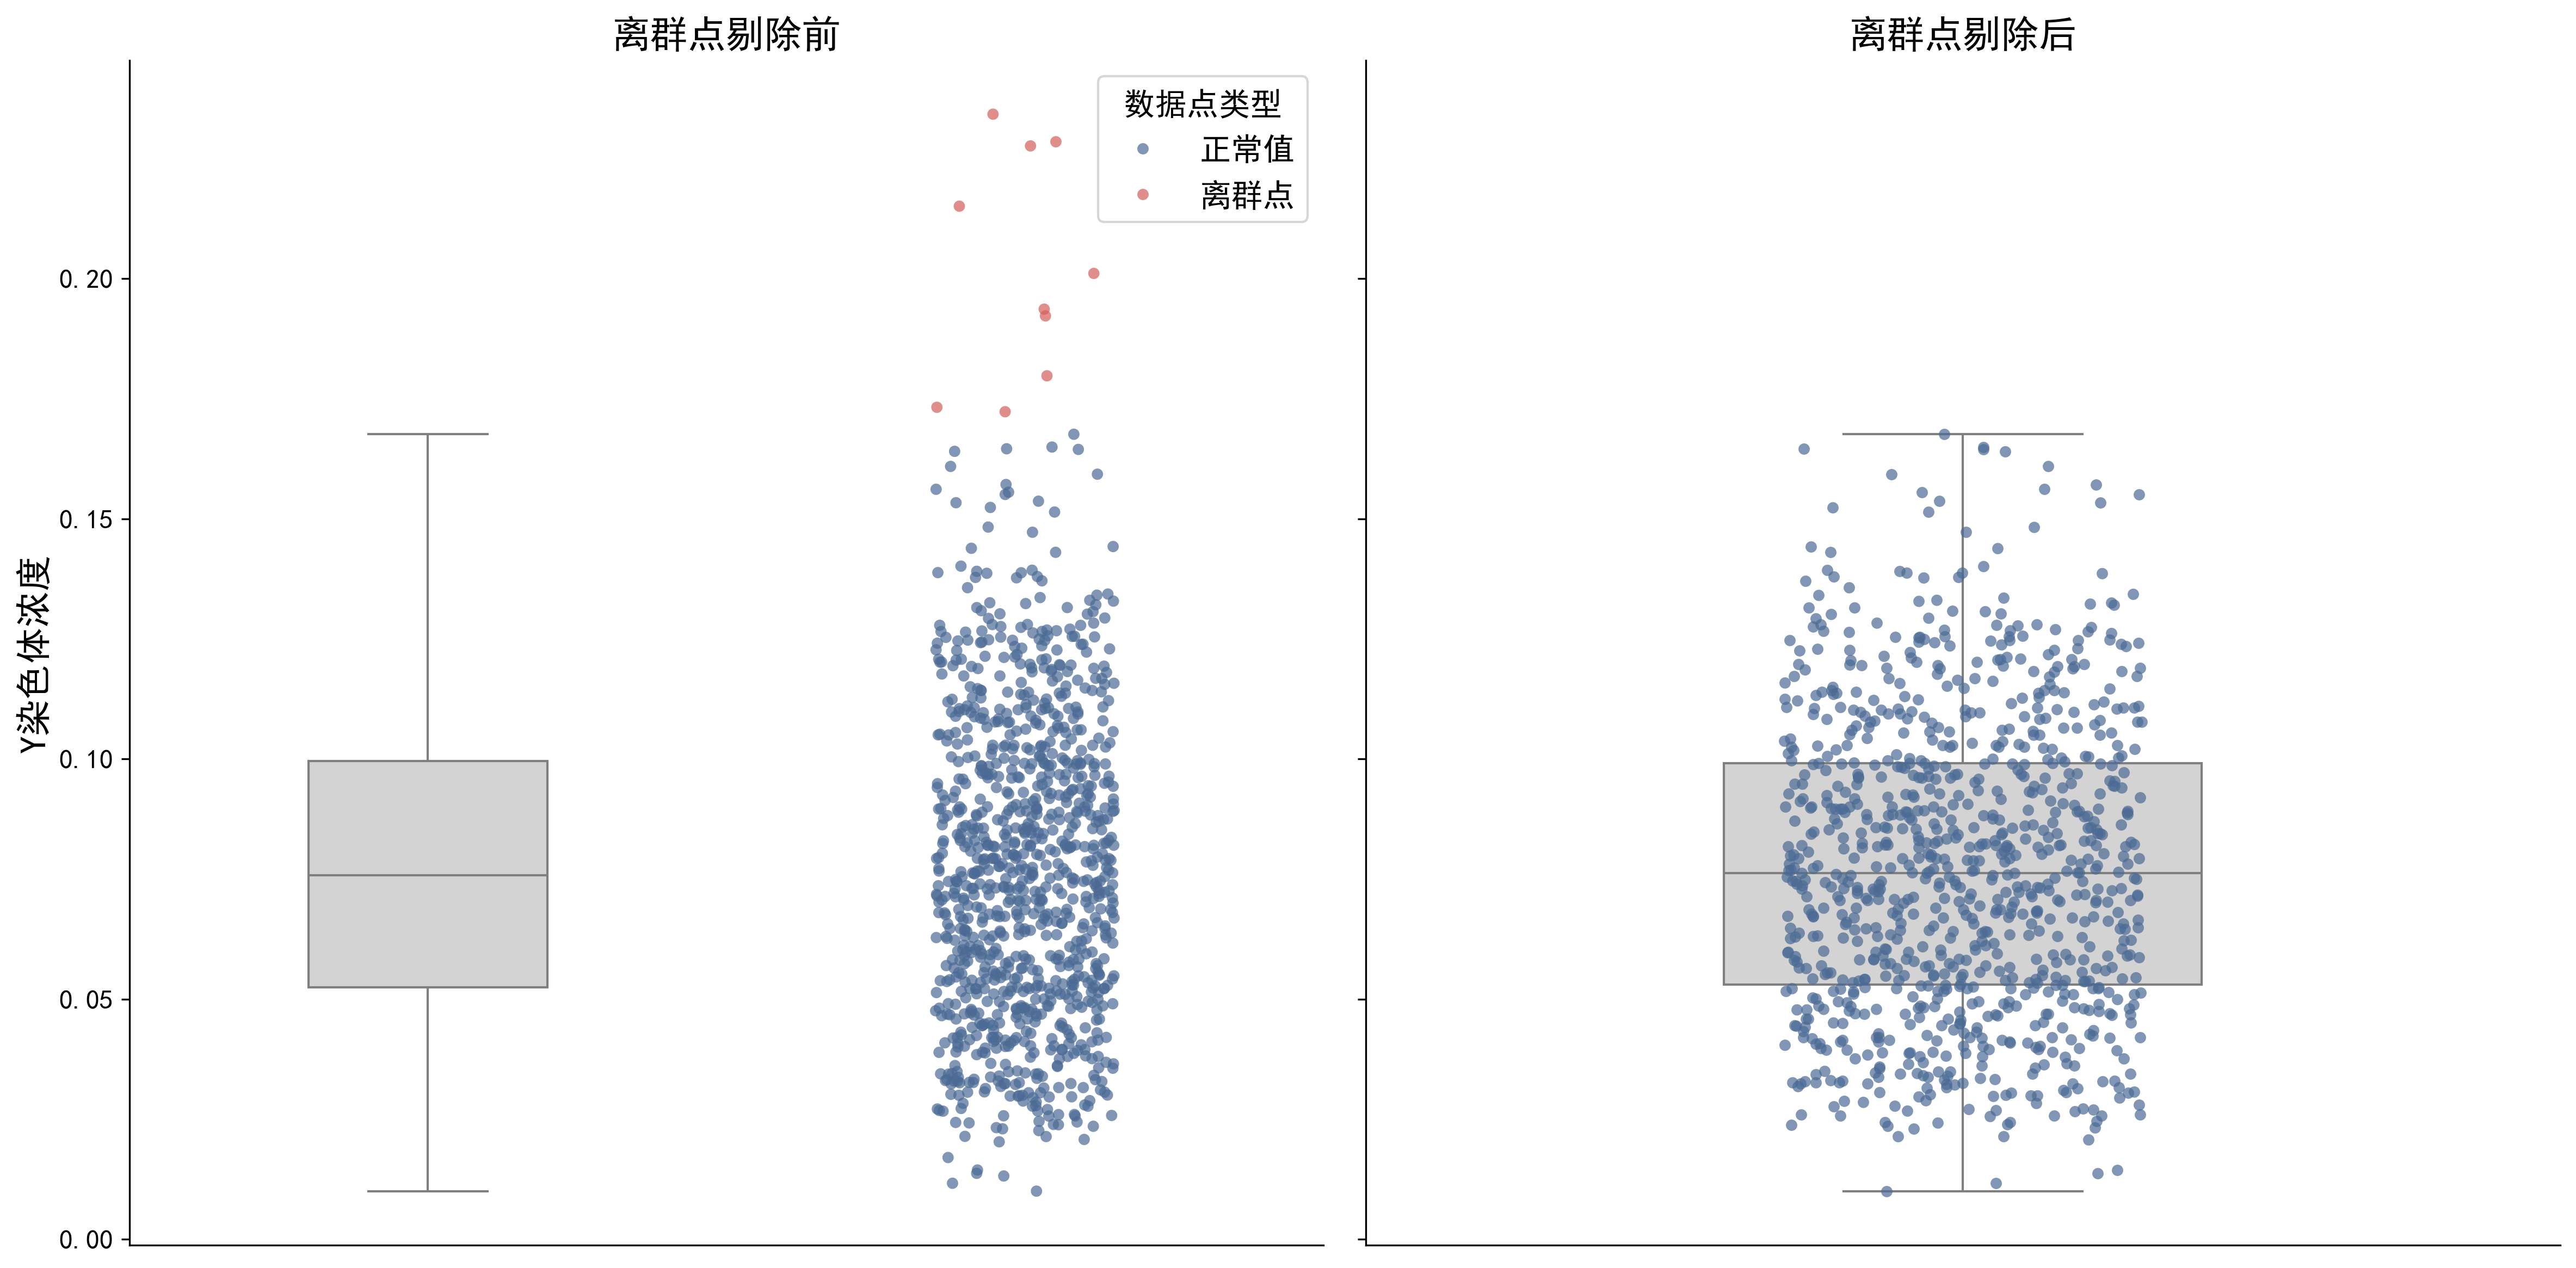
\includegraphics[width=\textwidth]{figs/3问题一/Y浓度离群点剔除可视化.png}
\caption{Y染色体浓度数据离群点剔除前后对比}
\label{fig:outlier_removal}
\end{figure}

\cref{fig:outlier_removal}为数据清洗过程的可视化结果,其对比了Y染色体浓度在离群点剔除前后的数据分布,被识别为离群点的数据点以不同颜色标记,清洗后的数据分布更为集中,减少了极端值对模型估计的潜在干扰。

在正式建模之前,我们对清洗后的数据进行了探索性分析。通过绘制Y染色体浓度与孕周、孕妇BMI的散点图,我们对变量间的关系形态进行了初步探查,如\cref{fig:scatter_plots}所示。

\begin{figure}[h!]
\centering
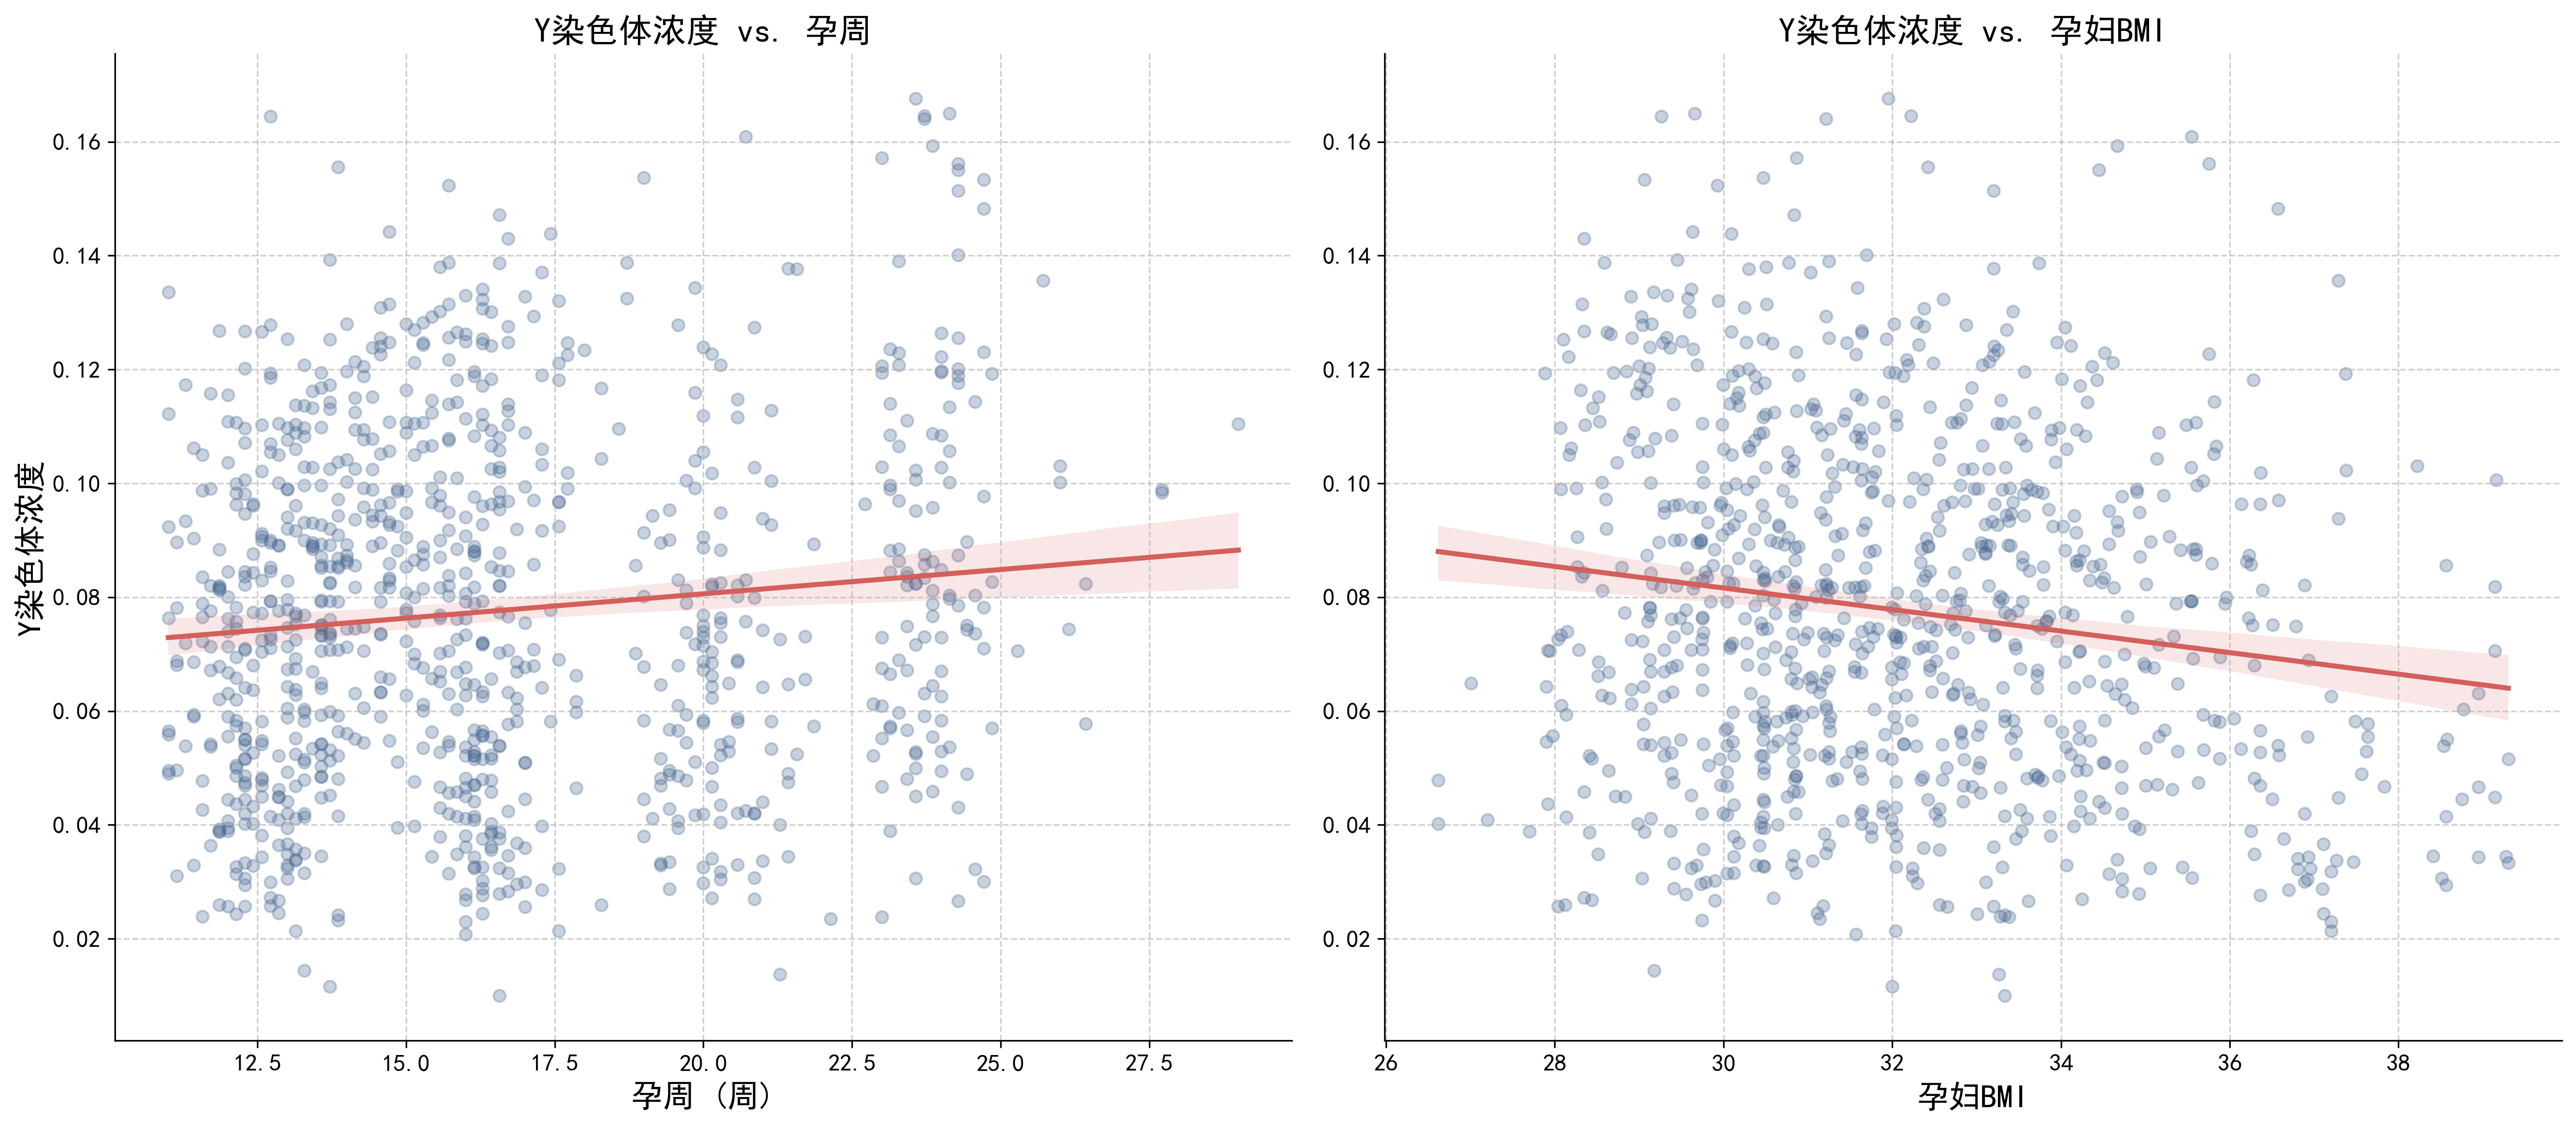
\includegraphics[width=1\textwidth]{figs/3问题一/Y浓度_vs_变量_散点图.png}
\caption{Y染色体浓度与孕周及BMI的散点关系图}
\label{fig:scatter_plots}
\end{figure}

根据\cref{fig:scatter_plots},Y染色体浓度与孕妇BMI的散点分布较为弥散,未呈现出特定的线性或非线性模式。而Y染色体浓度与孕周的散点图则呈现出一种微弱的U型曲线趋势,表明两者之间可能存在非线性关系。为量化变量间的关联强度,我们计算了皮尔逊与斯皮尔曼相关系数。皮尔逊相关系数用以衡量线性关联,其计算公式为
\begin{equation}
r = \frac{\sum_{i=1}^{n}(x_i - \bar{x})(y_i - \bar{y})}{\sqrt{\sum_{i=1}^{n}(x_i - \bar{x})^2} \sqrt{\sum_{i=1}^{n}(y_i - \bar{y})^2}}
\end{equation}

斯皮尔曼相关系数则用以衡量单调关系,计算公式为
\begin{equation}
\rho = 1 - \frac{6 \sum_{i=1}^{n} d_i^2}{n(n^2 - 1)}
\end{equation}

计算结果汇总于\cref{tab:correlation}。

\begin{table}[h!]
\centering
\caption{Y染色体浓度与孕周、BMI的相关性分析}
\label{tab:correlation}
\begin{tabular}{lcc}
\hline
变量对 & 皮尔逊相关系数 $r$ & 斯皮尔曼相关系数 $\rho$ \\
\hline
浓度 vs 孕周 & 0.1087 & 0.0851 \\
浓度 vs BMI & -0.1531 & -0.1321 \\
\hline
\end{tabular}
\end{table}

\cref{tab:correlation}的数据显示,Y染色体浓度与孕周、BMI的线性相关性均较弱,这与散点图的观察结果一致,并进一步说明简单的线性模型可能不足以描述变量间的复杂关系。

\subsection{关系模型的构建与择优}
基于探索性分析的发现,我们构建了四种不同复杂度的模型来拟合Y染色体浓度、孕周与BMI之间的关系,并通过统计指标对它们进行比较,以选取最合适的模型。

模型一为多元线性回归模型,作为后续比较的基准。其形式为
\begin{equation}
Y_{ij} = \beta_0 + \beta_1 GW_{ij} + \beta_2 BMI_{ij} + e_{ij}
\end{equation}

模型二为多元多项式回归模型,用以捕捉潜在的非线性关系。其形式为
\begin{equation}
Y_{ij} = \beta_0 + \sum_{k=1}^p \beta_k GW_{ij}^k + \sum_{l=1}^q \gamma_l BMI_{ij}^l + e_{ij}
\end{equation}

模型三为多元指数回归模型,通过对数变换处理可能的指数增长关系。其形式为
\begin{equation}
\ln(Y_{ij}) = \beta_0 + \beta_1 GW_{ij} + \beta_2 BMI_{ij} + e_{ij}
\end{equation}

考虑到数据中可能存在同一孕妇的多次检测记录,孕妇个体间的差异可能对Y染色体浓度有较大影响。因此,我们引入了非线性混合效应模型,即模型四。该模型在多项式回归的基础上,为每个孕妇个体设置了随机效应项,以解释个体间的异质性。其通用形式为
\begin{equation}
Y_{ij} = (\beta_0 + u_{0i}) + \sum_{k=1}^p \beta_k GW_{ij}^k + \sum_{l=1}^q \gamma_l BMI_{ij}^l + e_{ij}
\end{equation}
其中 $u_{0i}$ 服从均值为0的正态分布,代表第 $i$ 位孕妇的个体效应。

为在上述模型中进行选择,我们计算了各自的对数似然值、赤池信息准则AIC、贝叶斯信息准则BIC、均方根误差RMSE和决定系数$R^2$,评估指标对比见\cref{tab:model_comparison}。

\begin{table}[h!]
\centering
\caption{四种候选模型的评估指标对比}
\label{tab:model_comparison}
\resizebox{\columnwidth}{!}{
\begin{tabular}{lccccc}
\hline
模型 & 对数似然值 & AIC & BIC & RMSE & $R^2$ \\
\hline
M1 线性回归 & 1999.22 & -3992.43 & -3977.82 & 0.0303 & 0.0377 \\
M2 多项式回归 & 1999.61 & -3991.23 & -3971.75 & 0.0303 & 0.0375 \\
M3 指数回归 & -573.15 & 1152.29 & 1166.90 & 0.0310 & 0.0376\\
M4 混合效应模型 & 2367.64 & -4719.27 & -4680.32 & 0.0326 & 边际:0.4052, 条件:0.9160 \\
\hline
\end{tabular}}
\end{table}

\cref{tab:model_comparison}的评估结果显示,模型一、二、三的决定系数均低于0.04,说明这些模型对Y染色体浓度变异的解释能力非常有限。相比之下,模型四的对数似然值最高,AIC和BIC值最低,显示出更优的拟合度。

\begin{figure}[h!]
\centering
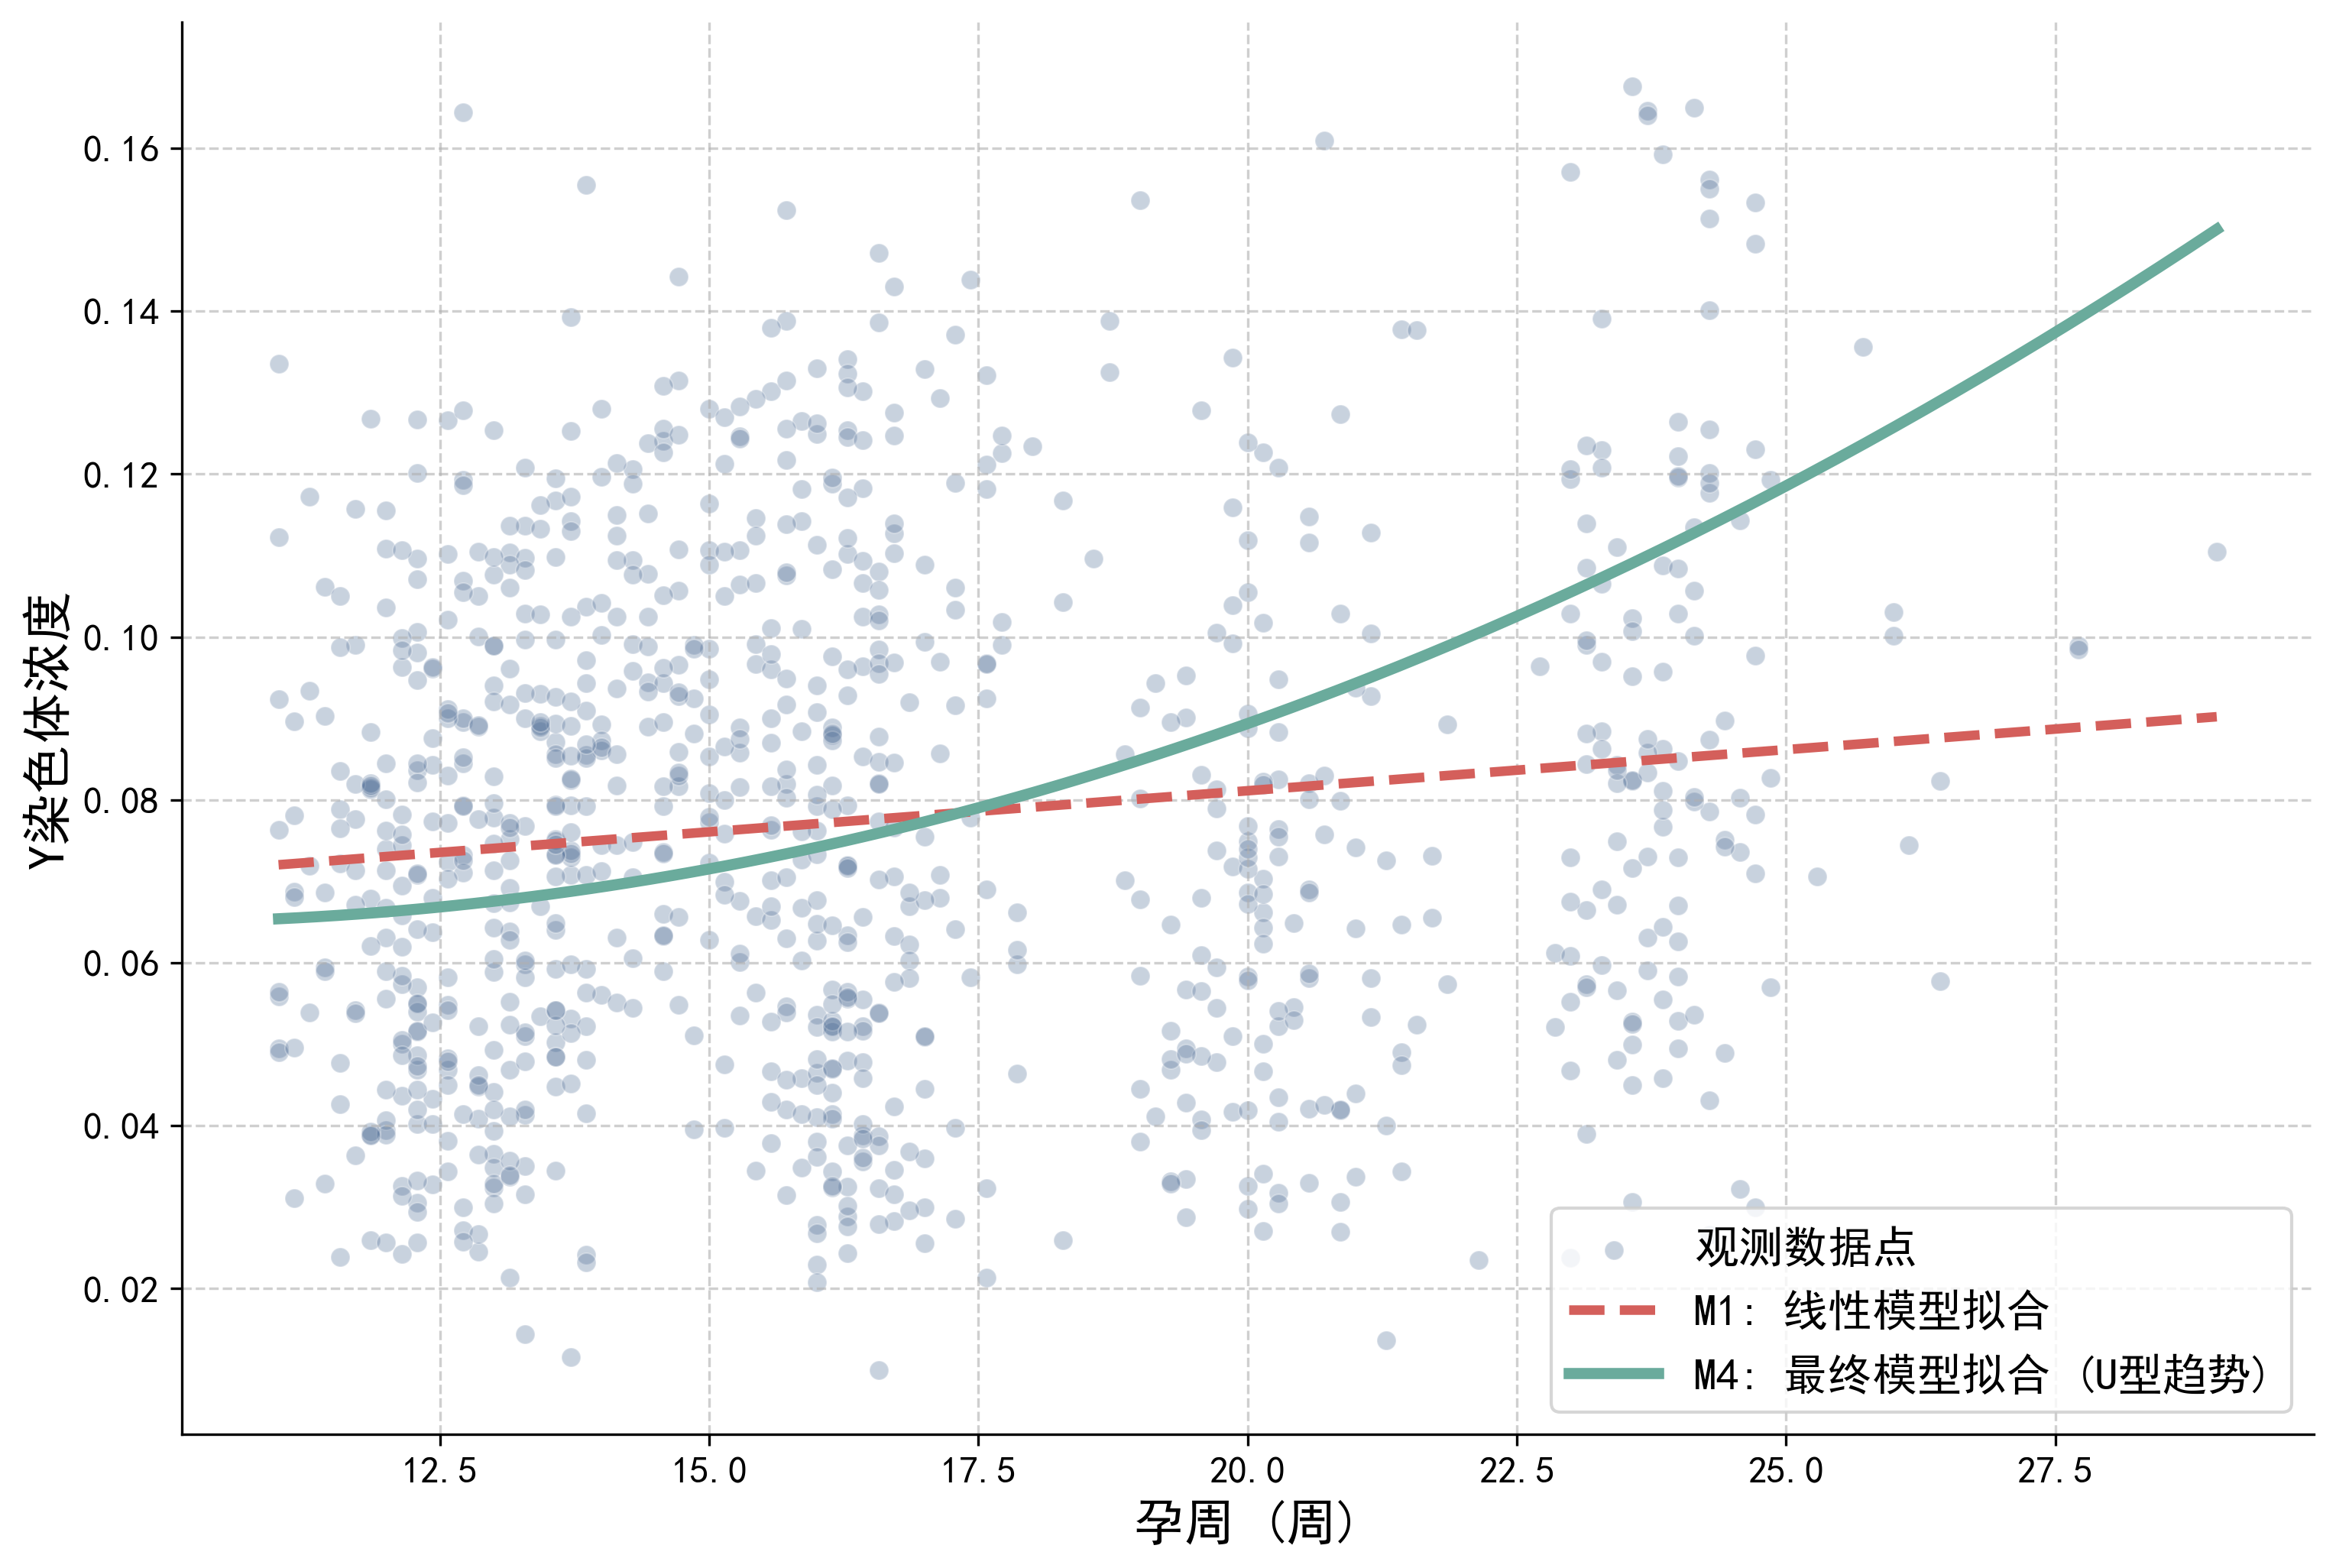
\includegraphics[width=0.9\textwidth]{figs/3问题一/模型拟合效果对比图.png}
\caption{线性模型与非线性混合效应模型拟合效果对比}
\label{fig:fit_comparison}
\end{figure}

\cref{fig:fit_comparison}对比了线性模型与非线性模型对数据趋势的拟合情况。非线性模型所捕捉的U型曲线趋势比线性模型更能贴合数据的整体分布形态。基于上述分析,我们最终选择非线性混合效应模型作为描述Y染色体浓度与母体指标关系的模型。

\subsection{最终模型解析与显著性检验}
在确定采用非线性混合效应模型后,我们通过似然比检验对其具体形式进行了优化。检验结果表明,在模型中加入孕周的二次项能提升模型拟合度,而加入BMI的二次项及孕周与BMI的交互项则无改善。因此,最终确立的模型形式为
\begin{equation}
Y_{ij} = (\beta_0 + u_{0i}) + ((\beta_1 + u_{1i})GW_{ij} + \beta_2 GW_{ij}^2) + \gamma_1 BMI_{ij} + e_{ij}
\end{equation}
其中,$u_{0i}$ 和 $u_{1i}$ 分别代表第 $i$ 位孕妇的随机截距和随机斜率。为检验模型中各变量的效应,我们对模型系数进行了t检验。其原假设为系数等于零,统计量计算公式为
\begin{equation}
t = \frac{\hat{\beta}_k - 0}{SE(\hat{\beta}_k)}
\end{equation}

同时,我们通过F检验来评估模型整体的显著性,其原假设为所有自变量系数同时为零,统计量计算公式为
\begin{equation}
F = \frac{SSR/k}{SSE/(n-k-1)}
\end{equation}

最终模型固定效应参数的估计与检验结果如\cref{tab:fixed_effects}所示。

\begin{table}[h!]
\centering
\small
\caption{最终模型固定效应参数估计与检验}
\label{tab:fixed_effects}
\begin{tabular}{lcccccc}
\hline
变量 & 系数 & 标准误 & z值 & p值 & 95\%置信区间下限 & 95\%置信区间上限 \\
\hline
Intercept & 0.1188 & 0.0217 & 5.471 & $<$0.001 & 0.0762 & 0.1613 \\
孕周 & -0.0044 & 0.0012 & -3.639 & 0.0003 & -0.0067 & -0.0020 \\
孕妇BMI & -0.0010 & 0.0006 & -1.670 & 0.0949 & -0.0022 & 0.0002 \\
孕周二次项 & 0.0002 & 3.47e-05 & 6.532 & $<$0.001 & 0.0002 & 0.0003 \\
\hline
\end{tabular}
\end{table}

\cref{tab:fixed_effects}的参数估计结果显示,孕周项的系数显著为负,而其二次项的系数显著为正,这共同确认了Y染色体浓度随孕周呈现先下降后上升的U型非线性关系。截距项也表现出高度显著性。孕妇BMI项的p值为0.0949,在0.05的显著性水平下不显著,表明其对Y染色体浓度的影响不稳定。

\begin{table}[h!]
\centering
\caption{最终模型决定系数}
\label{tab:r_squared}
\begin{tabular}{lc}
\hline
指标 & 值 \\
\hline
边际 $R^2$ & 0.4052 \\
条件 $R^2$ & 0.9160 \\
\hline
\end{tabular}
\end{table}

模型的决定系数分析见\cref{tab:r_squared}。边际$R^2$为0.4052,表示由孕周和BMI所代表的固定效应可以解释约40.5\%的变异。条件$R^2$为0.9160,表示在模型同时考虑固定效应和个体随机效应后,总共能解释91.6\%的变异。这两个$R^2$值的差异,印证了个体差异性在Y染色体浓度变化中起主导作用。

\begin{figure}[h!]
\centering
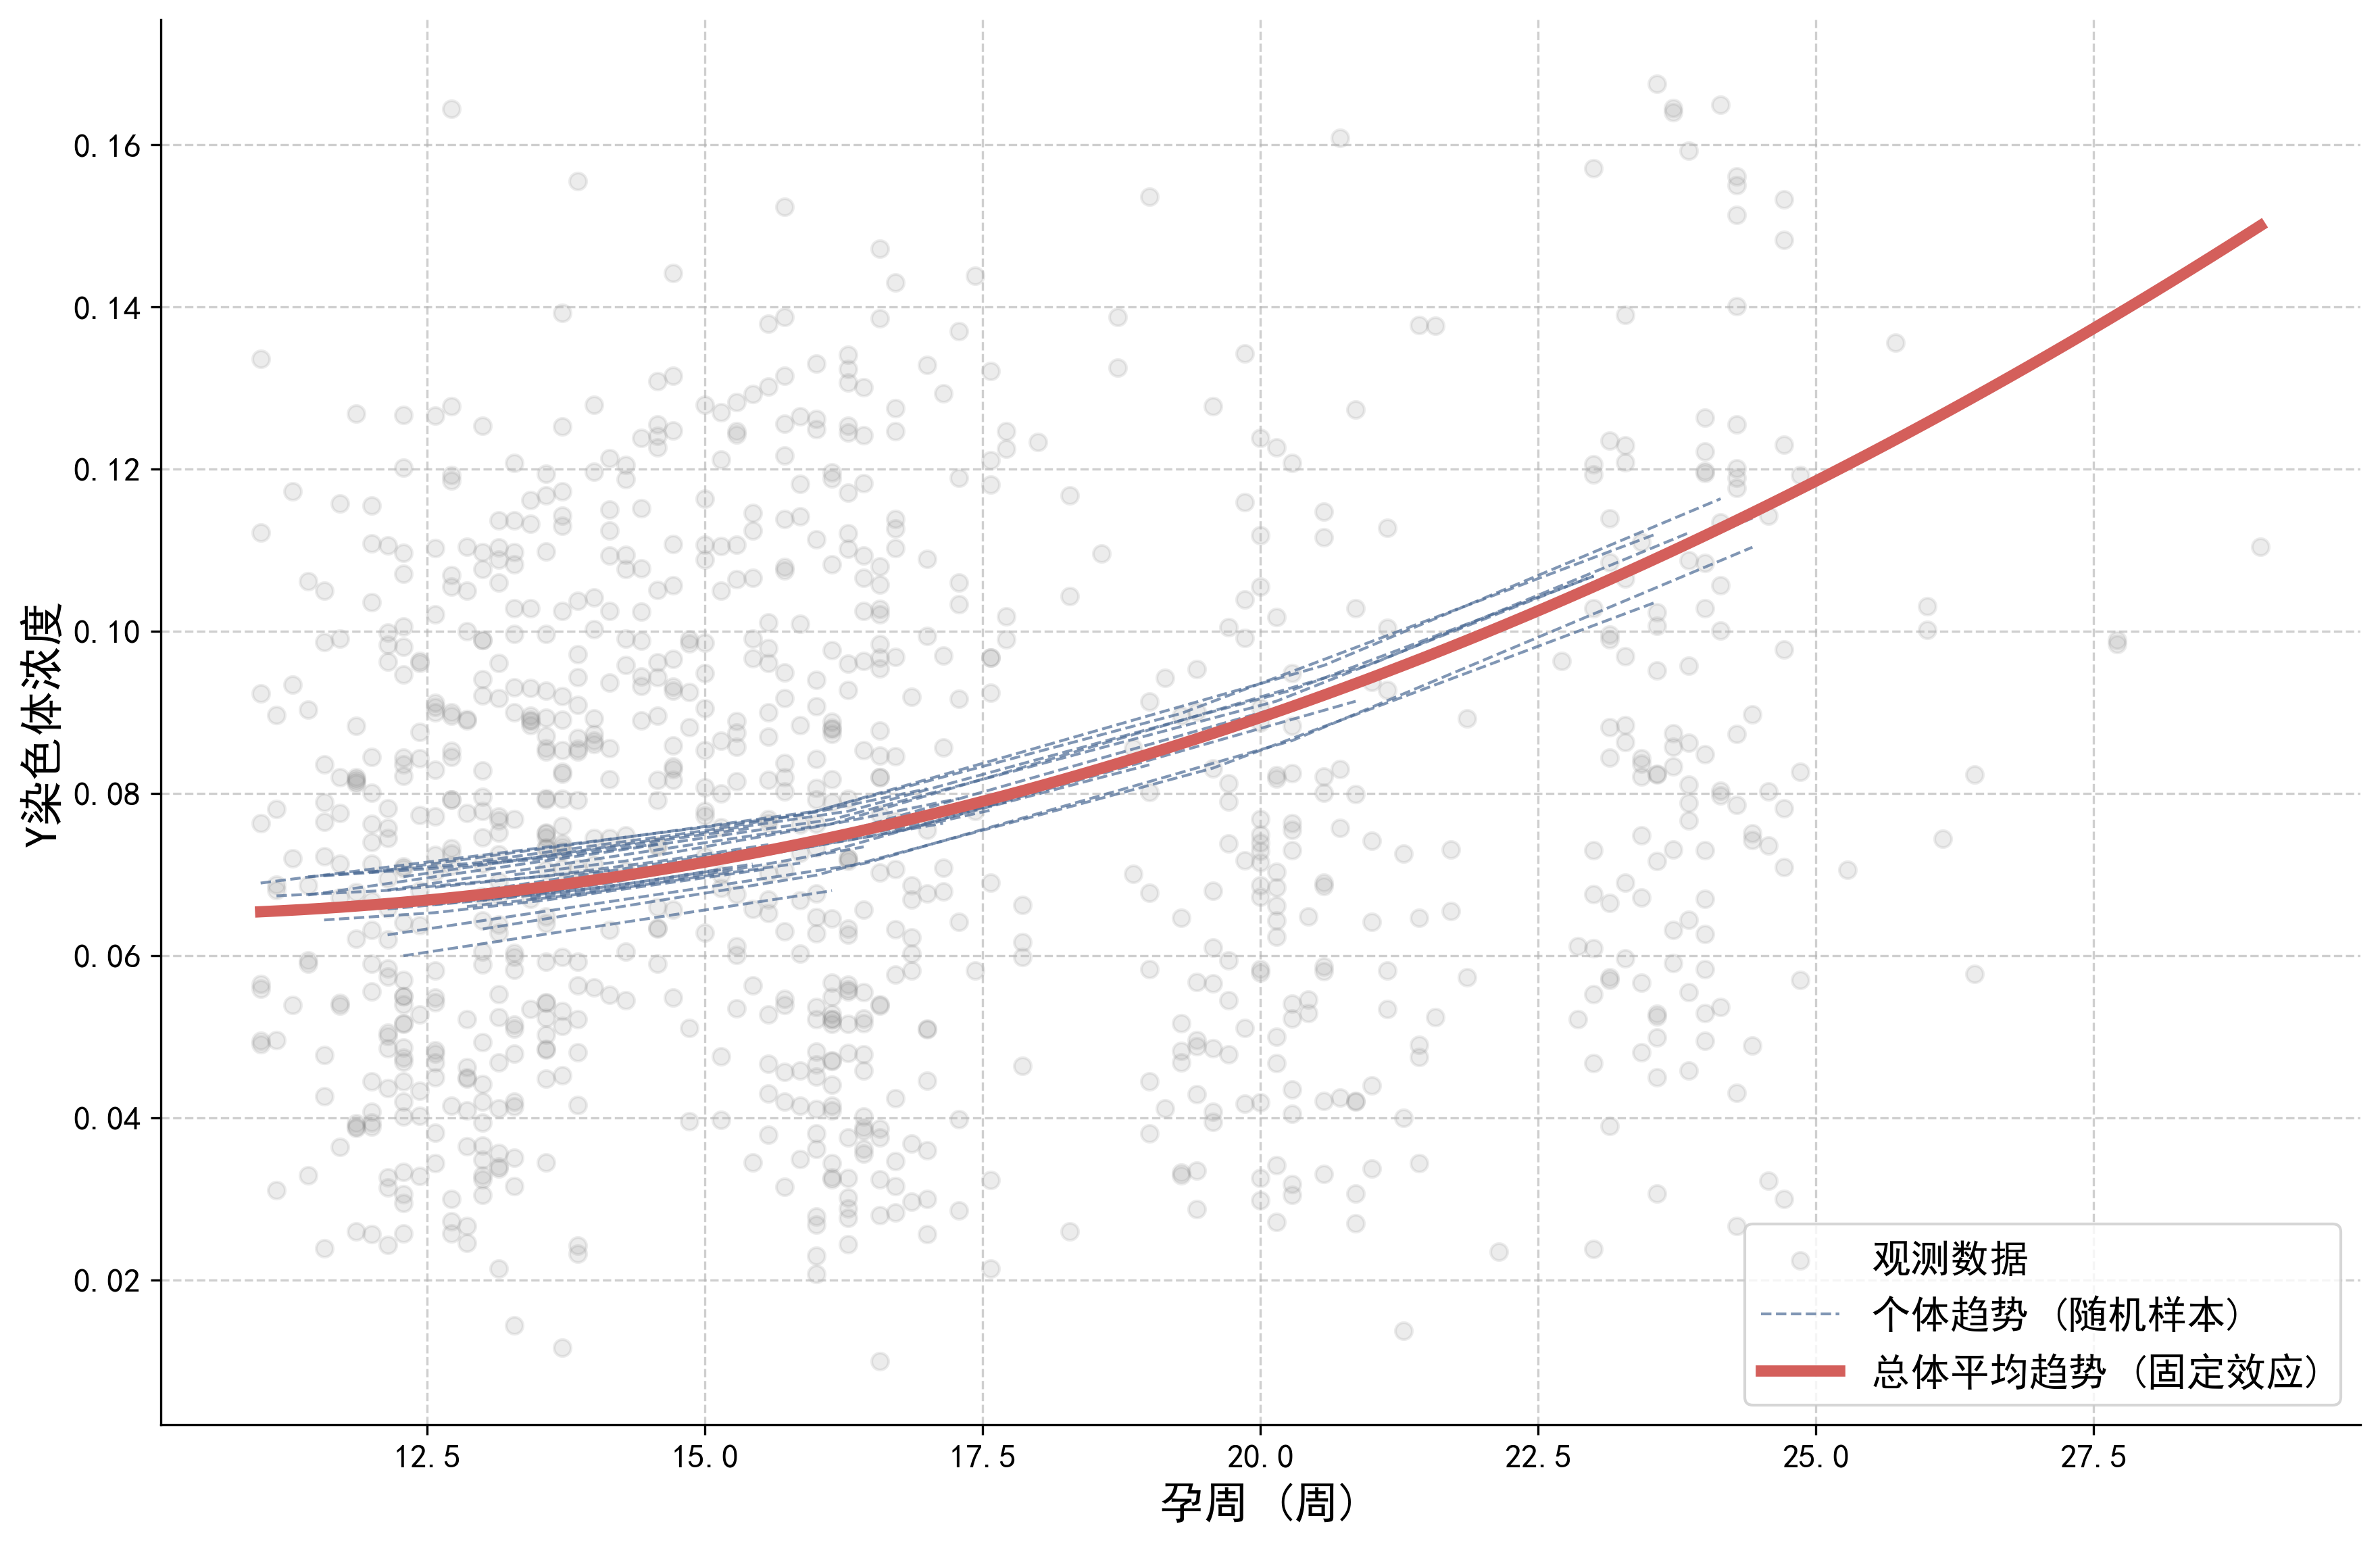
\includegraphics[width=\textwidth]{figs/3问题一/最终模型M4_可视化.png}
\caption{最终模型揭示的总体趋势与个体差异}
\label{fig:final_model_viz}
\end{figure}

\cref{fig:final_model_viz}是最终模型结果的可视化呈现。图中的红色实线代表了由固定效应决定的平均变化趋势,即总体样本共有的U型规律。大量的蓝色虚线则代表了考虑随机效应后,每一位孕妇个体的实际变化轨迹。

综合上述分析,可以得出Y染色体浓度变化规律的结论。其变化遵循一个由孕周主导的U型非线性模式,即浓度随孕周增加先发生下降,后转为上升,这一趋势具有统计学上的显著性。然而,这一普遍规律在不同孕妇个体间的表现存在巨大差异,个体独特性是引起浓度变化的更主要来源。相比之下,孕妇的BMI指标在此模型中未表现出稳定的影响。

\input{contents/4问题二}
\input{contents/5问题三}
\input{contents/6问题四}


\newpage

% 参考文献
\bibliographystyle{plain}
\bibliography{reference}

\newpage

\end{document}